\chapter{Mô hình hóa hệ thống}

\section{Use case diagram}
\begin{figure}[h]
    \centering
    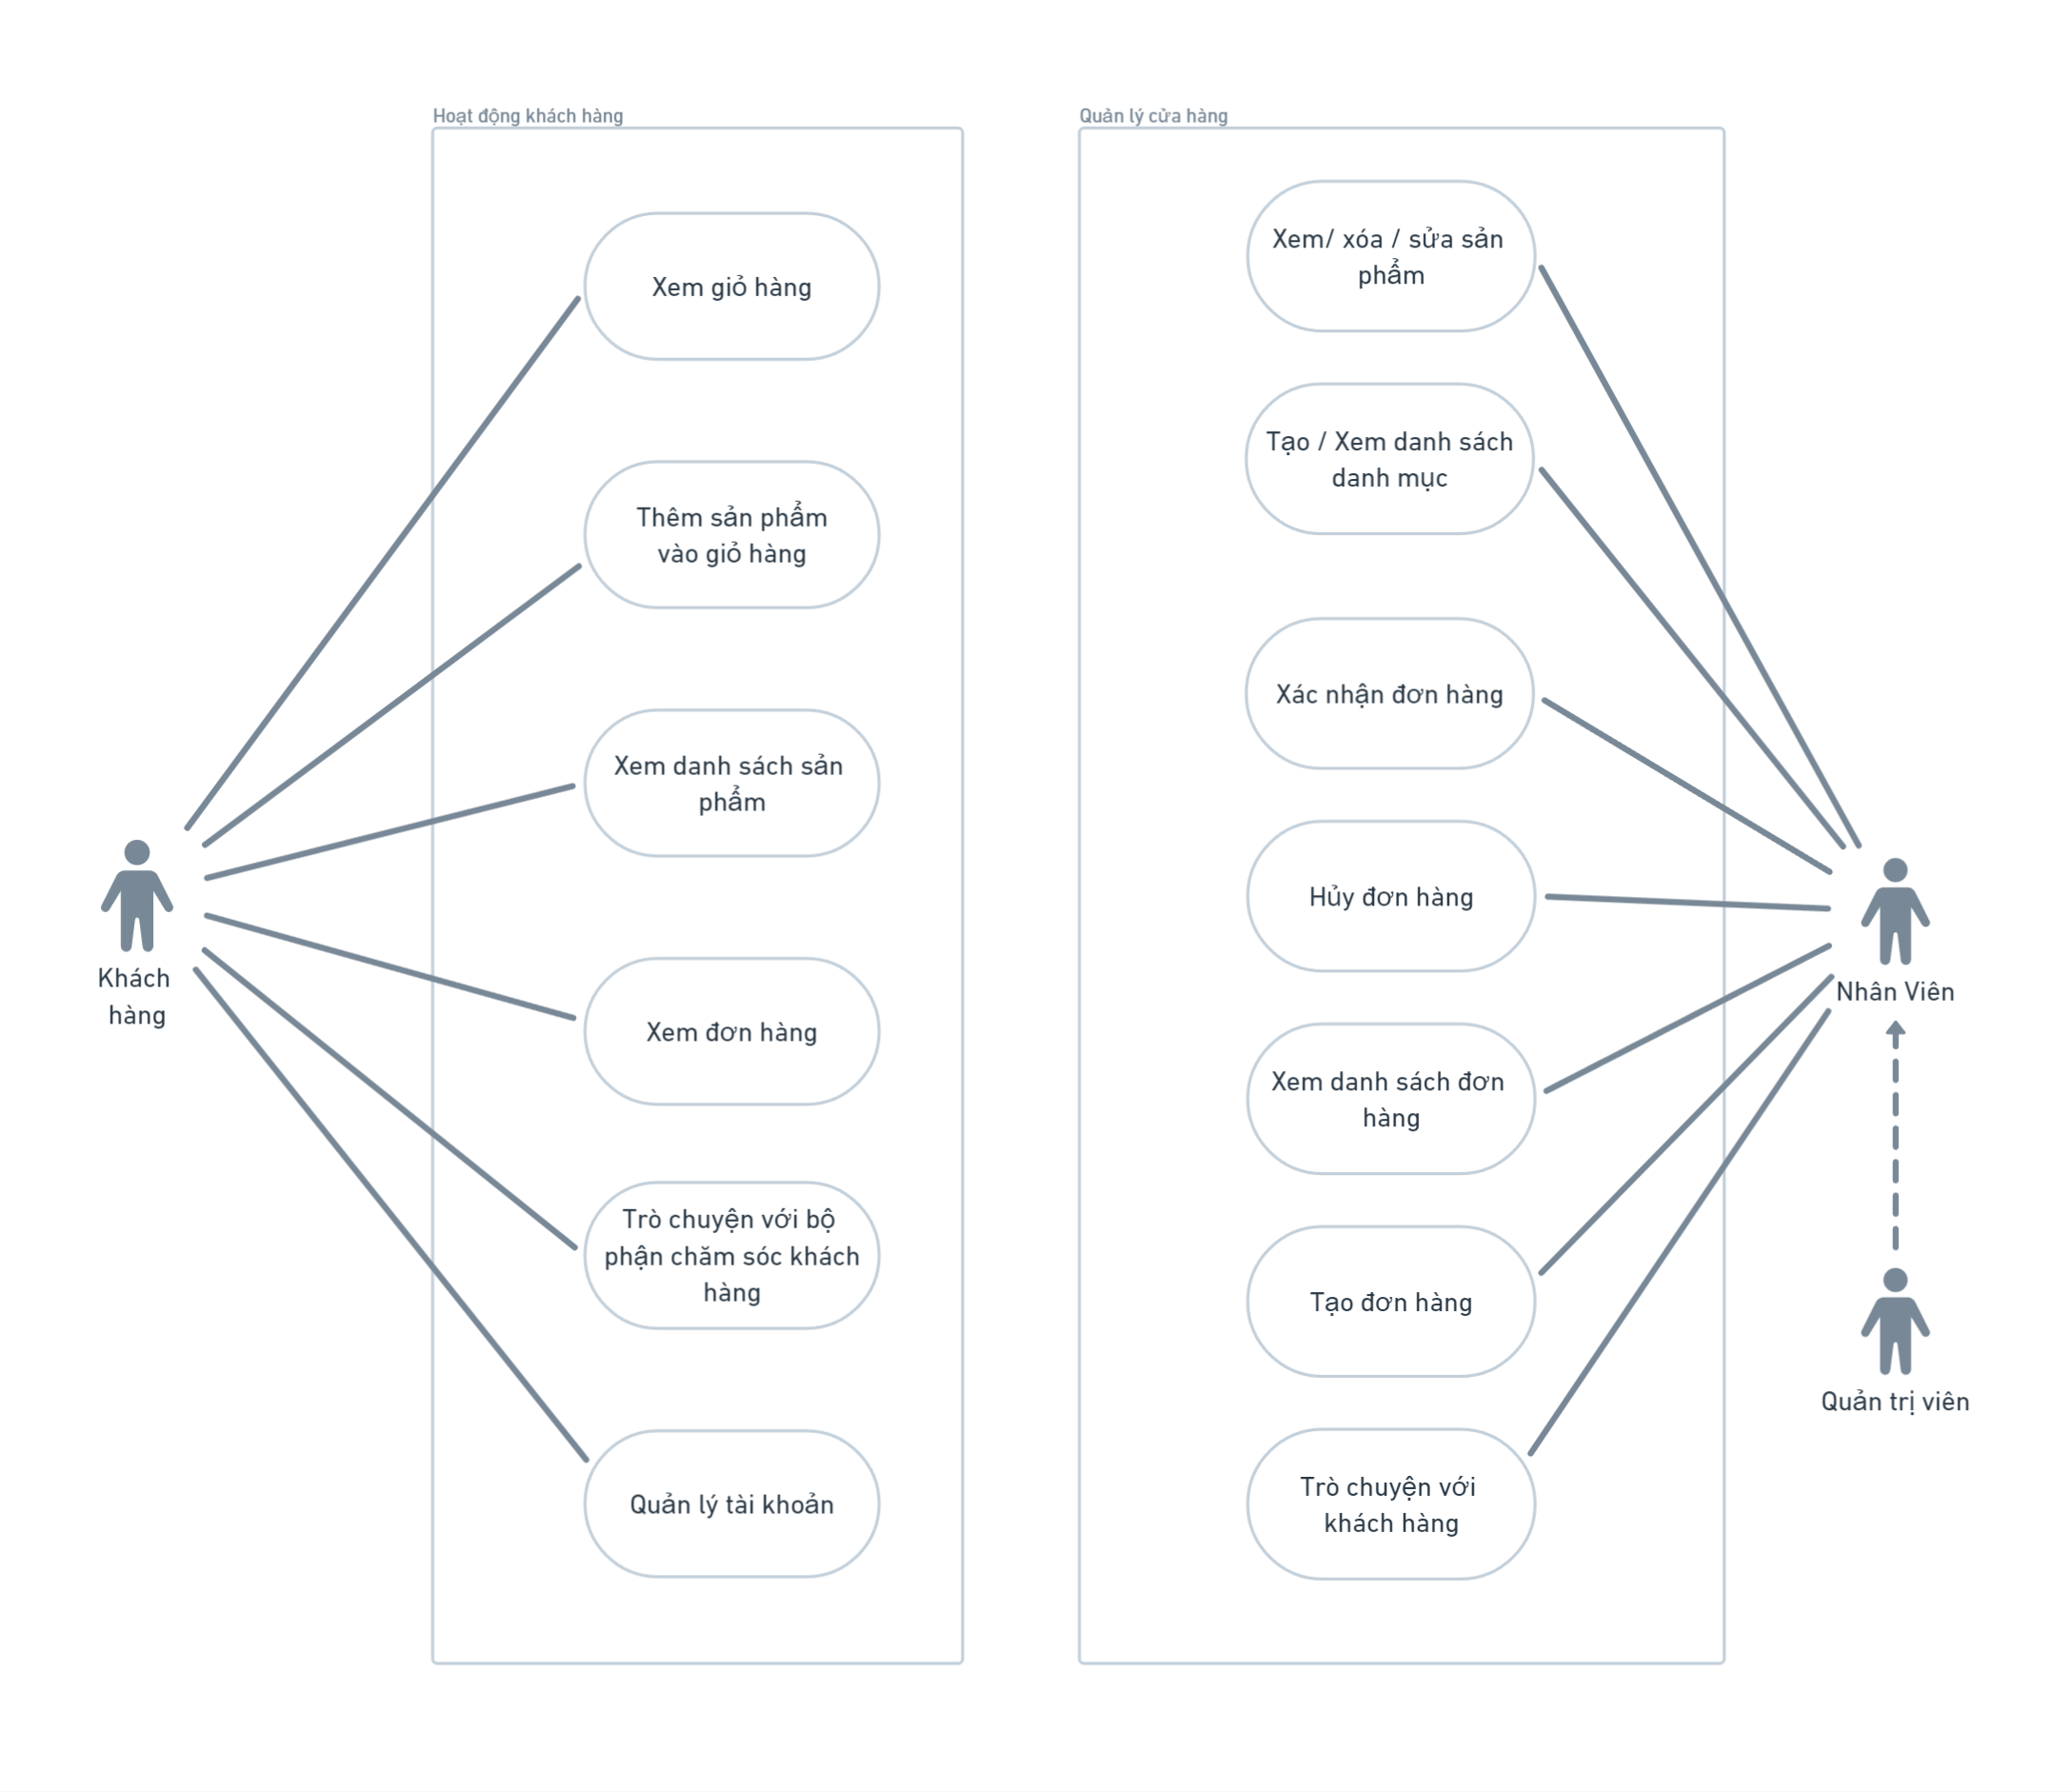
\includegraphics[scale = 0.22]{img/use-case.png}
    \caption{Use-case diagram cho toàn bộ hệ thống}
    \label{fig:taskAssignment}
\end{figure}
\newpage
\subsection{Module quản lý tài khoản}
\begin{figure}[h]
    \centering
    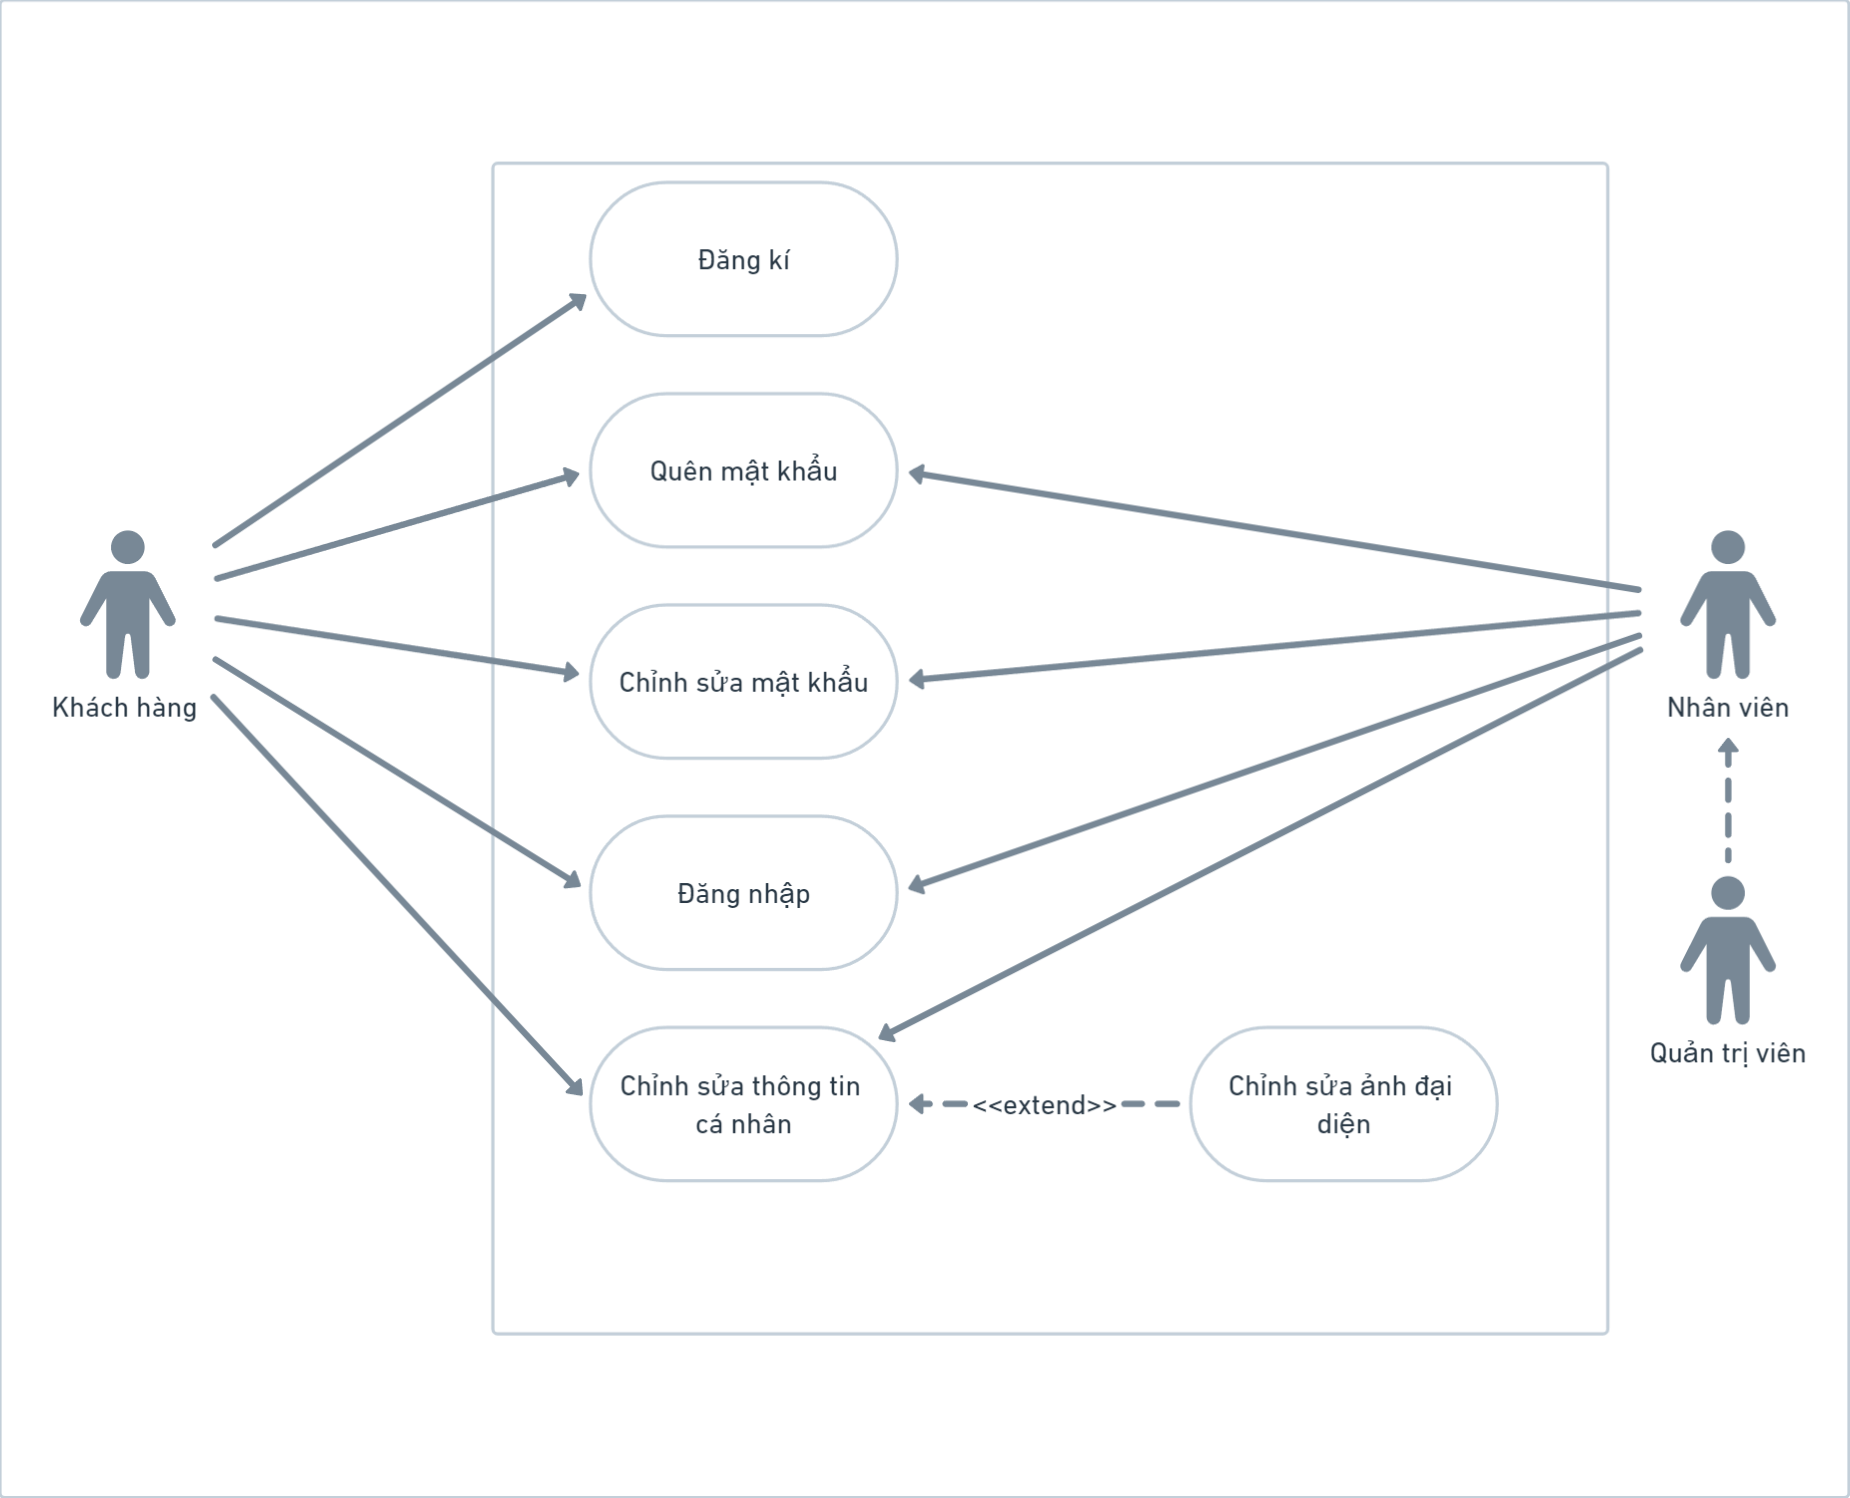
\includegraphics[scale = 0.2]{img/mod/tk-mod.png}
    \vspace{1cm}
    \caption{Use-case diagram cho module quản lý tài khoản}
    \label{fig:taskAssignment}
\end{figure}

\begin{longtable}{|>{\hspace{0pt}}m{0.15\linewidth}|>{\hspace{0pt}}m{0.79\linewidth}|} 
\hline
Usecase id & UC2.2.1 \endfirsthead 
\hline
Usecase name & Đăng ký \\ 
\hline
Actor & Khách hàng \\ 
\hline
Description & Người dùng đăng ký tài khoản cá nhân trên hệ thống \\ 
\hline
Trigger & Người dùng nhấn vào Đăng ký. \\ 
\hline
Pre-condition & 1. Có kết nối internet \\ 
\hline
Post-condition & 1. Tài khoản cá nhân của người dùng được tạo thành công.\par{}2. Người dùng có thể sử dụng tài khoản cá nhân để đăng nhập, sử dụng các chức năng cần tài khoản của hệ thống. \\ 
\hline
Normal Flow & 1. Người dùng nhấn vào đăng ký.\par{}2. Hệ thống chuyển hướng người dùng tới giao diện yêu cầu người dùng nhập số điện thoại đăng ký.\par{}3. Người dùng tiến hành nhập và xác nhận số điện thoại cần đăng ký.\par{}4. Hệ thống gửi mã OTP qua số điện thoại được nhập vào.~\par{}5. Người dùng nhận được mã OTP.\par{}6. Người dùng nhập mã OTP vừa nhận được.\par{}7. Hệ thống xác thực thông tin thành công và chuyển hướng người dùng tới giao diện hiện các trường thông tin cần thiết để người dùng nhập vào, bao gồm:~\par{}+ Các thông tin bắt buộc: mật khẩu, nhập lại mật khẩu, họ và tên, giới tính, địa chỉ (chi tiết đến ấp/thôn/khóm/tổ hoặc số nhà tên đường).\par{}+ Các thông tin không bắt buộc: email, ảnh đại diện, ngày sinh, số căn cước công dân.\par{}8. Người dùng nhập các thông tin.\par{}9. Người dùng chọn lệnh Hoàn thành đăng ký.\par{}10. Hệ thống xác thực thông tin thành công, tạo tài khoản cho người dùng thành công, hiển thị thông báo thành công và định hướng người dùng về trang đăng nhập. \\ 
\hline
Alternative Flows & Không \\ 
\hline
Exceptions & 4b. Hệ thống xác nhận số điện thoại này đã có người sử dụng, hiển thị thông báo.\par{}\textit{Use case tiếp tục Use case UC2.2.1-2}\par{}5b. Người dùng không nhận được mã OTP sau 60 giây.\par{}5b1. Người dùng chọn lệnh Gửi lại mã OTP.\par{}\textit{Use case tiếp tục Use case UC2.2.1-4}\par{}5b2. Người dùng chọn Nhập lại số điện thoại.\par{}\textit{Use case tiếp tục Use case UC2.2.1-3}\par{}7b. Hệ thống xác thực mã OTP không chính xác và hiển thị thông báo.\par{}7b1. Người dùng chọn nhập lại OTP.\par{}\textit{Use case tiếp tục Use case UC2.2.1-6}\par{}10b. Người dùng không nhập đủ các thông tin bắt buộc hoặc nhập thông tin không hợp lệ, hệ thống hiển thị thông báo yêu cầu nhập đầy đủ thông tin ở các trường.\par{}\textit{Use case tiếp tục Use case UC2.2.1-8} \\ 
\hline
Business rules & Không \\ 
\hline
Non functional-requirement & NFR2.2.1-1: Thời gian giữa mỗi lần người dùng gửi yêu cầu mã OTP là 60 giây.\par{}NFR2.2.1-2: Mật khẩu của người dùng phải được hash bằng MD5. \\ 
\hline
\caption{Use case scenario cho chức năng đăng kí}
\end{longtable}

%
%

\begin{longtable}{|>{\hspace{0pt}}m{0.206\linewidth}|>{\hspace{0pt}}m{0.735\linewidth}|} 
\hline
Usecase id & UC2.2.2 \endfirsthead 
\hline
Usecase name & Đăng nhập \\ 
\hline
Actor & Khách hàng, nhân viên, quản trị viên \\ 
\hline
Description & Người dùng đăng nhập vào hệ thống để sử dụng những tính năng của hệ thống \\ 
\hline
Trigger & Người dùng vào Đăng nhập \\ 
\hline
Pre-condition & 1. Có kết nối internet.\par{}2. Tài khoản của người dùng đã được tạo sẵn. \\ 
\hline
Post-condition & 1. Người dùng đăng nhập vào hệ thống thành công. \\ 
\hline
Normal Flow & 1. Người dùng truy cập vào hệ thống.\par{}2. Người dùng nhấn vào nút Đăng nhập.\par{}3. Người dùng nhập số điện thoại và mật khẩu đã đăng ký và chọn lệnh Đăng nhập.\par{}4. Hệ thống xác nhận thông tin đăng nhập thành công và cho phép người dùng đăng nhập vào hệ thống. \\ 
\hline
Alternative Flows & Không \\ 
\hline
Exceptions & 4b. Hệ thống xác thực thông tin đăng nhập không thành công và hiển thị thông báo.\par{}4b1. Người dùng chọn nhập lại thông tin.\par{}\textit{Use case tiếp tục UC2.2.2-3.}\par{}4b1. Người dùng chọn lệnh hủy đăng nhập.\par{}\textit{Use case dừng lại.}\par{}4b2. Người dùng chọn lệnh lấy lại mật khẩu.\par{}\textit{Use case tiếp tục use case UC2.2.2-3.~} \\ 
\hline
Business rules & Không \\ 
\hline
Non functional-requirement & NFR2.2.2-1: Timeout cho màn hình đăng nhập dưới 60 giây.\par{}NFR2.2.2-2: Mật khẩu của người dùng phải được hash bằng MD5. \\ 
\hline
\caption{Use case scenario cho chức năng đăng nhập}
\end{longtable}

% \usepackage{array}
% \usepackage{longtable}


\begin{longtable}{|>{\hspace{0pt}}m{0.163\linewidth}|>{\hspace{0pt}}m{0.779\linewidth}|} 
\hline
Usecase id & UC2.2.3 \endfirsthead 
\hline
Usecase name & Quên mật khẩu \\ 
\hline
Actor & Khách hàng, nhân viên, quản trị viên \\ 
\hline
Description & Người dùng quên mật khẩu và muốn đặt lại mật khẩu để đăng nhập vào hệ thống \\ 
\hline
Trigger & Người dùng vào Quên mật khẩu~ \\ 
\hline
Pre-condition & 1. Có kết nối internet\par{}2. Tài khoản của người dùng đã được tạo sẵn \\ 
\hline
Post-condition & 1. Người dùng đặt lại mật khẩu cho tài khoản thành công \\ 
\hline
Normal Flow & 1. Người dùng nhấn vào nút Quên mật khẩu.\par{}2. Hệ thống chuyển hướng người dùng tới giao diện yêu cầu người dùng nhập số điện thoại đã dùng để đăng ký.\par{}3. Người dùng tiến hành nhập và xác nhận số điện thoại cần đặt lại mật khẩu.\par{}4. Hệ thống gửi mã OTP qua số điện thoại được nhập vào.~\par{}5. Người dùng nhận được mã OTP.\par{}6. Người dùng nhập mã OTP vừa nhận được.\par{}7. Hệ thống xác thực thông tin thành công và chuyển hướng người dùng tới giao diện đặt lại mật khẩu, gồm trường mật khẩu và nhập lại mật khẩu.\par{}8. Người dùng nhập mật khẩu và nhập lại mật khẩu.\par{}9. Người dùng chọn lệnh Đặt lại mật khẩu.\par{}10. Hệ thống xác thực thông tin thành công và hiển thị thông báo thành công, chuyển hướng người dùng về trang đăng nhập. \\ 
\hline
Alternative Flows & Không \\ 
\hline
Exceptions & 5b. Người dùng không nhận được mã OTP sau 60 giây.\par{}5b1. Người dùng chọn lệnh Gửi lại mã OTP.\par{}\textit{Use case tiếp tục Use case UC2.2.3-4}\par{}5b2. Người dùng chọn lệnh Nhập lại số điện thoại.\par{}\textit{Use case tiếp tục Use case UC2.2.3-3}\par{}7b. Hệ thống xác thực mã OTP không chính xác và hiển thị thông báo.\par{}7b1. Người dùng chọn nhập lại OTP.\par{}\textit{Use case tiếp tục Use case UC2.2.3-6}\par{}10b. Hệ thống xác nhận thông tin không trùng khớp, hiển thị thông báo mật khẩu không trùng khớp, yêu cầu người dùng thay đổi lại thông tin.\par{}\textit{Use case tiếp tục Use case UC2.2.3-8} \\ 
\hline
Business rules & Không \\ 
\hline
Non functional-requirement & NFR2.2.3-1: Thời gian giữa mỗi lần người dùng gửi yêu cầu mã OTP là 60 giây.\par{}NFR2.2.3-2: Mật khẩu của người dùng phải được hash bằng MD5. \\ 
\hline
\caption{Use case scenario cho chức năng quên mật khẩu}
\end{longtable}

\begin{longtable}{|>{\hspace{0pt}}m{0.169\linewidth}|>{\hspace{0pt}}m{0.773\linewidth}|} 
\hline
Usecase id & UC2.2.5 \endfirsthead 
\hline
Usecase name & Chỉnh sửa mật khẩu \\ 
\hline
Actor & Khách hàng, nhân viên, quản trị \\ 
\hline
Description & Người dùng muốn chỉnh sửa mật khẩu~ \\ 
\hline
Trigger & Người dùng nhấn vào Đổi mật khẩu \\ 
\hline
Pre-condition & 1. Có kết nối internet.\par{}2. Người dùng đã đăng nhập thành công.\par{}3. Người dùng đang ở trang thông tin cá nhân. \\ 
\hline
Post-condition & 1. Người dùng chỉnh sửa mật khẩu thành công. Hệ thống lưu lại mật khẩu mới của người dùng. \\ 
\hline
Normal Flow & 1. Người dùng nhấn vào Đổi mật khẩu.\par{}2. Hệ thống chuyển hướng người dùng tới giao diện đặt lại mật khẩu, gồm trường mật khẩu và nhập lại mật khẩu.\par{}3. Người dùng nhập mật khẩu và nhập lại mật khẩu.\par{}4. Người dùng chọn lệnh Đặt lại mật khẩu.\par{}5. Hệ thống xác thực thông tin thành công và hiển thị thông báo thành công, chuyển hướng người dùng về trang chủ. \\ 
\hline
Alternative Flows & Không \\ 
\hline
Exceptions & 5b. Hệ thống xác nhận thông tin không trùng khớp, hiển thị thông báo mật khẩu không trùng khớp, yêu cầu người dùng thay đổi lại thông tin.\par{}\textit{Use case tiếp tục Use case UC2.2.5-3} \\ 
\hline
Business rules & Không \\ 
\hline
Non functional-requirement & Không \\ 
\hline
\caption{Use case scenario cho chức năng Chỉnh sửa mật khẩu}
\end{longtable}

% \usepackage{array}
% \usepackage{longtable}


\begin{longtable}{|>{\hspace{0pt}}m{0.175\linewidth}|>{\hspace{0pt}}m{0.767\linewidth}|} 
\hline
Usecase id & UC2.2.6 \endfirsthead 
\hline
Usecase name & Chỉnh sửa thông tin cá nhân \\ 
\hline
Actor & Khách hàng, nhân viên, quản trị \\ 
\hline
Description & Người dùng thay đổi lại thông tin cá nhân tài khoản \\ 
\hline
Trigger & Người dùng vào Chỉnh sửa thông tin cá nhân \\ 
\hline
Pre-condition & 1. Có kết nối internet.\par{}2. Người dùng đã đăng nhập thành công.\par{}3. Người dùng đang ở trang thông tin cá nhân. \\ 
\hline
Post-condition & 1. Người dùng chỉnh sửa lại thông tin cá nhân thành công. Hệ thống lưu lại thông tin cá nhân mới của người dùng. \\ 
\hline
Normal Flow & 1. Người dùng nhấn vào nút Chỉnh sửa thông tin.\par{}2. Hệ thống chuyển hướng người dùng tới giao diện hiện các trường thông tin để người dùng có thể sửa các thông tin muốn thay đổi.\par{}3. Người dùng nhập các trường có thông tin cần thay đổi.\par{}4. Người dùng chọn lệnh “Lưu”.\par{}5. Hệ thống xác thực thông tin hợp lệ và hiển thị thông báo thành công, chuyển hướng người dùng về lại trang thông tin cá nhân. \\ 
\hline
Alternative Flows & Không \\ 
\hline
Exceptions & 5b. Hệ thống xác thực thông tin không hợp lệ, hiển thị thông báo ở các trường không hợp lệ.\par{}\textit{Use case tiếp tục UC2.2.6-3} \\ 
\hline
Business rules & Không \\ 
\hline
Non functional-requirement & NFR2.2.6-1: Mật khẩu của người dùng phải được hash bằng MD5. \\ 
\hline
\caption{Use case scenario cho chức năng chỉnh sửa thông tin cá nhân}
\end{longtable}

% \usepackage{array}
% \usepackage{longtable}

\begin{longtable}{|>{\hspace{0pt}}m{0.235\linewidth}|>{\hspace{0pt}}m{0.708\linewidth}|} 
\hline
Usecase id & UC2.2.7 \endfirsthead 
\hline
Usecase name & Chỉnh sửa ảnh đại diện \\ 
\hline
Actor & Khách hàng, nhân viên, quản trị \\ 
\hline
Description & Người dùng muốn chỉnh sửa ảnh đại diện \\ 
\hline
Trigger & Người dùng nhấn vào ảnh đại diện \\ 
\hline
Pre-condition & 1. Có kết nối internet.\par{}2. Người dùng đã đăng nhập thành công.\par{}3. Người dùng đang ở trang thông tin cá nhân. \\ 
\hline
Post-condition & 1. Người dùng chỉnh sửa ảnh đại diện thành công. \par{}2. Hệ thống lưu lại thay đổi về ảnh đại diện của người dùng. \\ 
\hline
Normal Flow & 1. Người dùng nhấn vào khung ảnh đại diện.\par{}2. Người dùng nhấn vào Chỉnh sửa ảnh đại diện. \par{}3. Hệ thống hiện Browser các file trên máy cá nhân người dùng. \par{}4. Người dùng chọn file ảnh mình muốn. \par{}5. Người dùng chọn xác nhận. \par{}6. Hệ thống xác nhận thông tin thành công, hiển thị hình đại diện mới của người dùng \\ 
\hline
Alternative Flows & 2b. Người dùng nhấn vào Xóa ảnh đại diện\par{}2b1. Hệ thống hiển thị thông báo yêu cầu người dùng xác nhận.\par{}2b2. Người dùng nhấn nút Xác nhận.\par{}2b3. Hệ thống xác nhận thông tin thành công, xóa ảnh đại diện của người dùng.~ \\ 
\hline
Exceptions & 6b. Hệ thống xác nhận file không phù hợp, hiển thị thông báo cho người dùng.\par{}\textit{Use case tiếp tục Use case UC2.2.7-2} \\ 
\hline
Business rules & Không \\ 
\hline
Non functional-requirement & Không \\ 
\hline
\caption{Use case scenario cho chức năng chỉnh sửa ảnh đại diện}
\end{longtable}

\newpage
\subsection{Module mua hàng}
\begin{figure}[h]
    \centering
    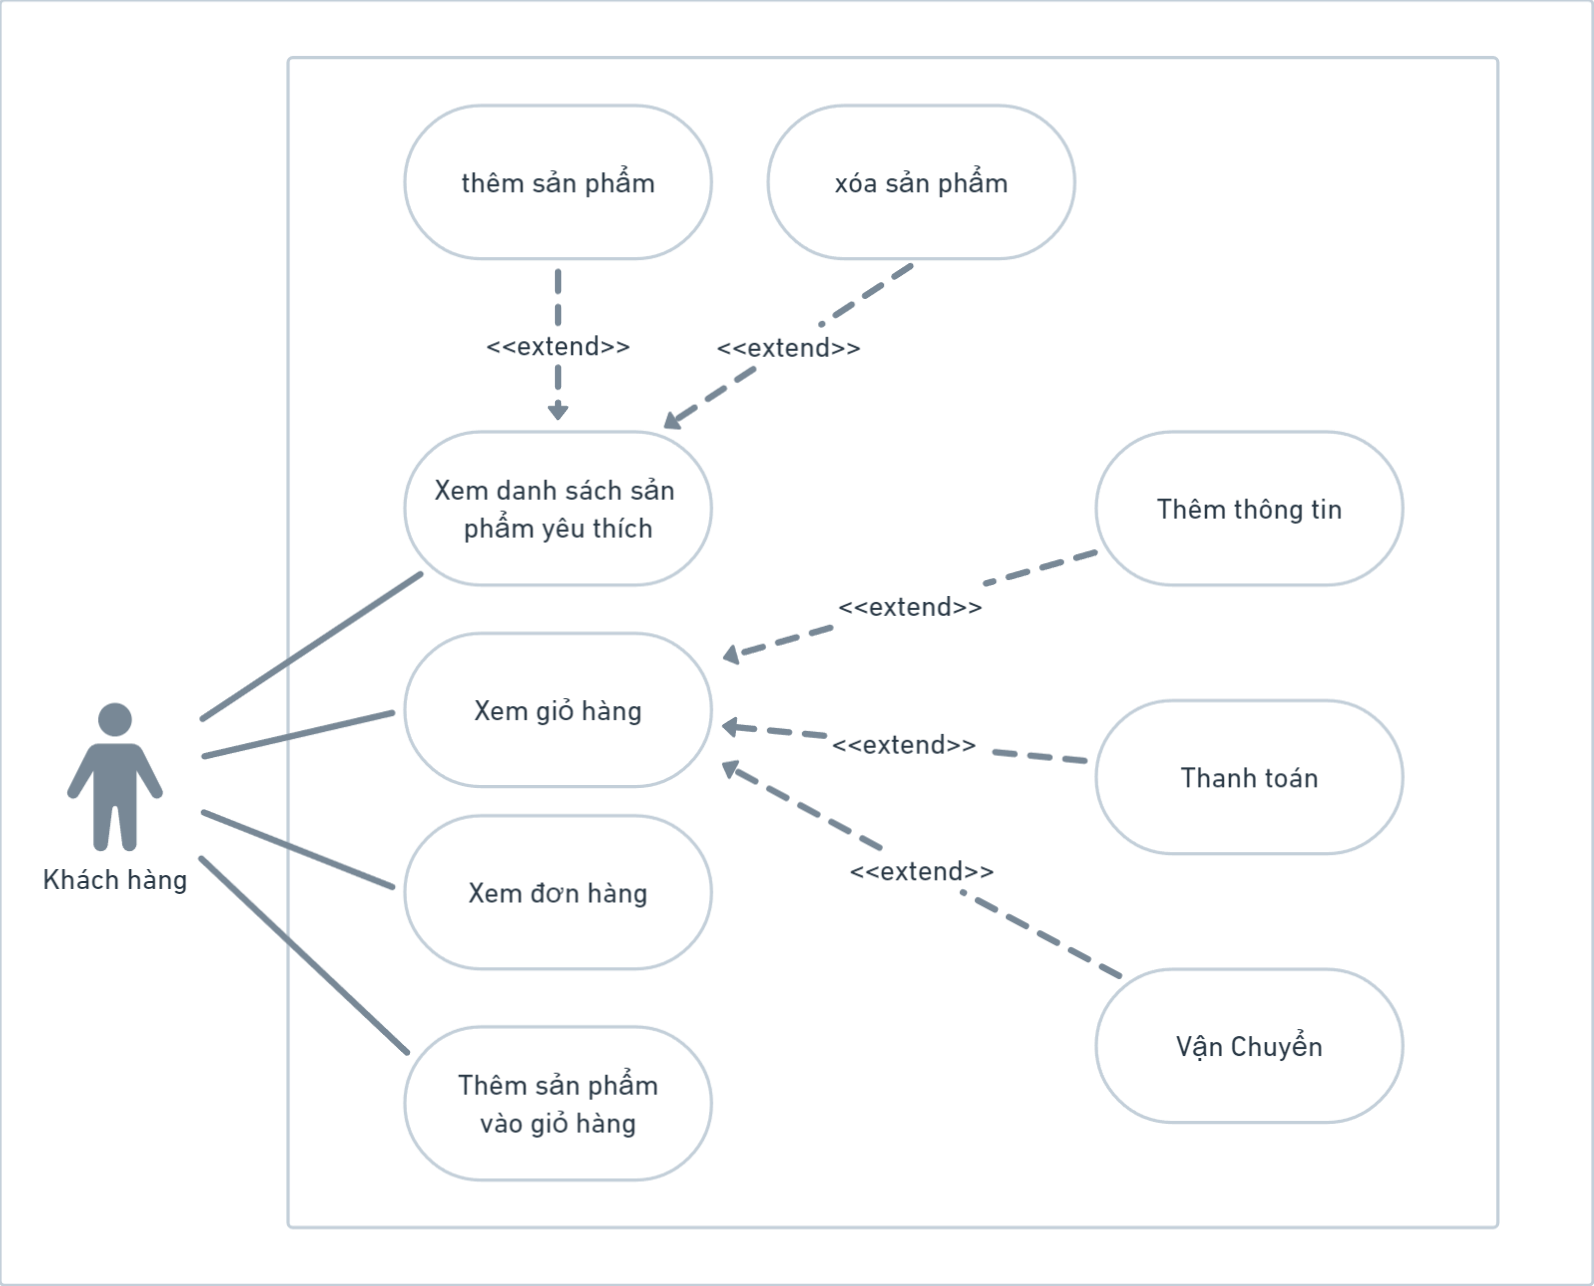
\includegraphics[scale = 0.2]{img/mod/mh-mod.png}
    \vspace{1cm}
    \caption{Use-case diagram cho module mua hàng}
    \label{fig:taskAssignment}
\end{figure}


% USECASE : XEM LỊCH SỬ MUA HÀNG
\begin{longtable}{|>{\hspace{0pt}}m{0.163\linewidth}|>{\hspace{0pt}}m{0.779\linewidth}|} 
\hline
Usecase id & UC2.3.1 \endfirsthead 
\hline
Usecase name & Xem đơn hàng \\ 
\hline
Actor & Khách hàng\\ 
\hline
Description & Người dùng, khách hàng muốn xem lại lịch sử mua hàng \\ 
\hline
Trigger & Người dùng, khách hàng vào mục lịch sử mua hàng~ \\ 
\hline
Pre-condition & 1. Có kết nối internet\par{}2. Tài khoản của người dùng đã được tạo sẵn \\ 
\hline
Post-condition & 1. Người dùng xem được lịch sử mua hàng \\ 
\hline
Normal Flow & 1. Người dùng/khách hàng vào mục xem lịch sử mua hàng ở mục dropdown trên thanh navbar.
\par{}2. Hệ thống chuyển người dùng tới trang lịch sử mua hàng.
\par{}3. Khách hàng/người dùng tùy chọn xem chi tiết đơn hàng.
 
\\ 
\hline
Alternative Flows & 
\par{}2a. Người dùng/ Khách hàng chưa đăng nhập.
\par{}2a1. Hệ thống chuyển người dùng tới trang đăng nhập/đăng kí.
\par{}2a2. Sau khi đăng nhập thành công, hệ thống chuyển tới trang lịch sử mua hàng.
\\ 
\hline
Exceptions & 
2b. Người dùng chưa có tài khoản đăng nhập
\par{}\textit{Use case tiếp tục tại Use case UC2.2.1}
\\
\hline
Business rules & Không \\ 
\hline
Non functional-requirement & Không \\ 
\hline
\caption{Use case scenario cho chức năng Xem lịch sử mua hàng}
\end{longtable}

% \usepackage{array}
% \usepackage{longtable}

% \usepackage{array}
% \usepackage{longtable}

% \begin{longtable}{|>{\hspace{0pt}}m{0.24\linewidth}|>{\hspace{0pt}}m{0.7\linewidth}|} 
% \hline
% Usecase id & UC1.8 \endfirsthead 
% \hline
% Usecase name & Xem lịch sử đơn hàng \\ 
% \hline
% Actor & Khách hàng \\ 
% \hline
% Description & Người dùng muốn xem lịch sử, chi tiết thông tin đơn hàng \\ 
% \hline
% Trigger & Người dùng nhấn vào phần Lịch sử đơn hàng \\ 
% \hline
% Pre-condition & 1. Có kết nối internet.\par{}2. Người dùng đã đăng nhập thành công. \\ 
% \hline
% Post-condition & 1. Người dùng xem được các thông tin về lịch sử đơn hàng \\ 
% \hline
% Normal Flow & 1. Người dùng nhấn vào Lịch sử đơn hàng\par{}2. Hệ thống chuyển người dùng đến trang hiển thị danh sách các đơn hàng đã mua\par{}2.1 Người dùng nhấn vào đơn hàng muốn xem để xem chi tiết đơn hàng. \\ 
% \hline
% Alternative Flows & Không~ \\ 
% \hline
% Exceptions & Không \\ 
% \hline
% Business rules & Không \\ 
% \hline
% Non functional-requirement & Không \\ 
% \hline

% \end{longtable}

% \usepackage{array}
% \usepackage{longtable}

\begin{longtable}{|>{\hspace{0pt}}m{0.229\linewidth}|>{\hspace{0pt}}m{0.713\linewidth}|} 
\hline
Usecase id & UC2.3.2 \endfirsthead 
\hline
Usecase name & Xem danh sách sản phẩm yêu thích \\ 
\hline
Actor & Khách hàng \\ 
\hline
Description & Người dùng muốn xem danh sách các sản phẩm yêu thích \\ 
\hline
Trigger & Người dùng nhấn vào Yêu thích \\ 
\hline
Pre-condition & 1. Có kết nối internet.\par{}2. Người dùng đã đăng nhập thành công. \\ 
\hline
Post-condition & 1. Người dùng xem được danh sách các sản phẩm yêu thích \\ 
\hline
Normal Flow & 1. Người dùng nhấn vào Yêu thích.\par{}2. Hệ thống chuyển người dùng đến trang hiển thị các sản phẩm được lọc theo Yêu thích.\par{}2.1 Người dùng nhấn vào sản phẩm muốn xem để xem chi tiết sản phẩm. \\ 
\hline
Alternative Flows & Không~ \\ 
\hline
Exceptions & Không \\ 
\hline
Business rules & Không \\ 
\hline
Non functional-requirement & Không \\ 
\hline
\caption{Use case scenario cho chức năng xem danh sách sản phẩm yêu thích}

\end{longtable}

% \usepackage{array}
% \usepackage{longtable}

% \begin{longtable}{|>{\hspace{0pt}}m{0.213\linewidth}|>{\hspace{0pt}}m{0.729\linewidth}|} 
% \hline
% Usecase id & UC2.3.3 \endfirsthead 
% \hline
% Usecase name & Xem lịch sử đánh giá sản phẩm \\ 
% \hline
% Actor & Khách hàng \\ 
% \hline
% Description & Người dùng muốn xem lịch sử đánh giá sản phẩm \\ 
% \hline
% Trigger & Người dùng nhấn vào Đánh giá \\ 
% \hline
% Pre-condition & 1. Có kết nối internet.\par{}2. Người dùng đã đăng nhập thành công. \\ 
% \hline
% Post-condition & 1. Người dùng xem được các đánh giá đã đăng. \\ 
% \hline
% Normal Flow & 1. Người dùng nhấn vào Đánh giá.\par{}2. Hệ thống chuyển người dùng đến trang hiển thị các đánh giá người dùng đã đăng.\par{}2.1 Người dùng nhấn vào đánh giá muốn xem để xem đánh giá tại trang thông tin chi tiết sản phẩm. \\ 
% \hline
% Alternative Flows & Không~ \\ 
% \hline
% Exceptions & Không \\ 
% \hline
% Business rules & Không \\ 
% \hline
% Non functional-requirement & Không \\ 
% \hline

% \end{longtable}

% \begin{longtable}{|>{\hspace{0pt}}m{0.213\linewidth}|>{\hspace{0pt}}m{0.729\linewidth}|} 
% \hline
% Usecase id & UC2.3.4 \endfirsthead 
% \hline
% Usecase name & Xem Chi tiết sản phẩm \\ 
% \hline
% Actor & Khách hàng \\ 
% \hline
% Description & Người dùng muốn xem chi tiết sản phẩm \\ 
% \hline
% Trigger & Người dùng nhấn vào sản phẩm \\ 
% \hline
% Pre-condition & 1. Có kết nối internet. \\ 
% \hline
% Post-condition & 1. Người dùng xem được chi tiết sản phẩm \\ 
% \hline
% Normal Flow & 1. Người dùng nhấn vào mục sản phẩm cụ thể.\par{}2. Hệ thống chuyển người dùng đến trang chi tiết sản phẩm \\ 
% \hline
% Alternative Flows & Không~ \\ 
% \hline
% Exceptions & Không \\ 
% \hline
% Business rules & Không \\ 
% \hline
% Non functional-requirement & Không \\ 
% \hline

% \end{longtable}

\begin{longtable}{|>{\hspace{0pt}}m{0.213\linewidth}|>{\hspace{0pt}}m{0.729\linewidth}|} 
\hline
Usecase id & UC2.3.3 \endfirsthead 
\hline
Usecase name & Thêm vào giỏ hàng \\ 
\hline
Actor & Khách hàng \\ 
\hline
Description & Người dùng muốn xem chi tiết sản phẩm \\ 
\hline
Trigger & Người dùng nhấn vào icon thêm vào giỏ hàng ở trang sản phẩm hoặc ở trong chi tiết sản phẩm \\ 
\hline
Pre-condition & 1. Có kết nối internet. \\
& 2. Người dung đã đăng nhập\\ 
\hline
Post-condition & 1. Người dùng thêm được sản phẩm vào trong giỏ hàng cá nhân \\ 
\hline
Normal Flow & 1. Người dùng chọn "thêm vào giỏ hàng" ở ô sản phẩm.\par{}2. Hệ thống thêm sản phẩm đã chọn vào giỏ hàng \\ 
\hline
Alternative Flows & 1a. Người dùng chọn xem chi tiết sản phẩm \\ 
& 1a1. Người dùng chọn "thêm vào giỏ hàng" ở mục chi tiết sản phẩm \\
\hline
Exceptions & Không \\ 
\hline
Business rules & Không \\ 
\hline
Non functional-requirement & Không \\ 
\hline
\caption{Use case scenario cho chức năng thêm vào giở hàng}
\end{longtable}

\begin{longtable}{|>{\hspace{0pt}}m{0.213\linewidth}|>{\hspace{0pt}}m{0.729\linewidth}|} 
\hline
Usecase id & UC2.3.4 \endfirsthead 
\hline
Usecase name & Xem giỏ hàng \\ 
\hline
Actor & Khách hàng \\ 
\hline
Description & Người dùng muốn xem giỏ hàng chứa các sản phẩm mình đã chọn \\ 
\hline
Trigger & Người dùng nhấn vào icon giỏ hàng \\ 
\hline
Pre-condition & 1. Có kết nối internet. \\
& 2. Người dung đã đăng nhập\\ 
\hline
Post-condition & 1. Người dùng nhấn vào icon giỏ hàng trên trang chủ \\ 
\hline
Normal Flow & 1. Người dùng nhấn vào icon giỏ hàng .\par{}2. Hệ thống popup ra trang hiển thị giỏ hàng. \\ 
\hline
Alternative Flows & 1a. Người dùng nhấn vào icon giỏ hàng ở trang danh sách sản phẩm \\ 
& 1b. Người dùng nhấn vào icon giỏ hàng trang chi tiết sản phẩm \\
\hline
Exceptions & Không \\ 
\hline
Business rules & Không \\ 
\hline
Non functional-requirement & Không \\ 
\hline
\caption{Use case scenario cho chức năng xem giỏ hàng}

\end{longtable}

\newpage
\subsection{Module quản lý đơn hàng}
\begin{figure}[h]
    \centering
    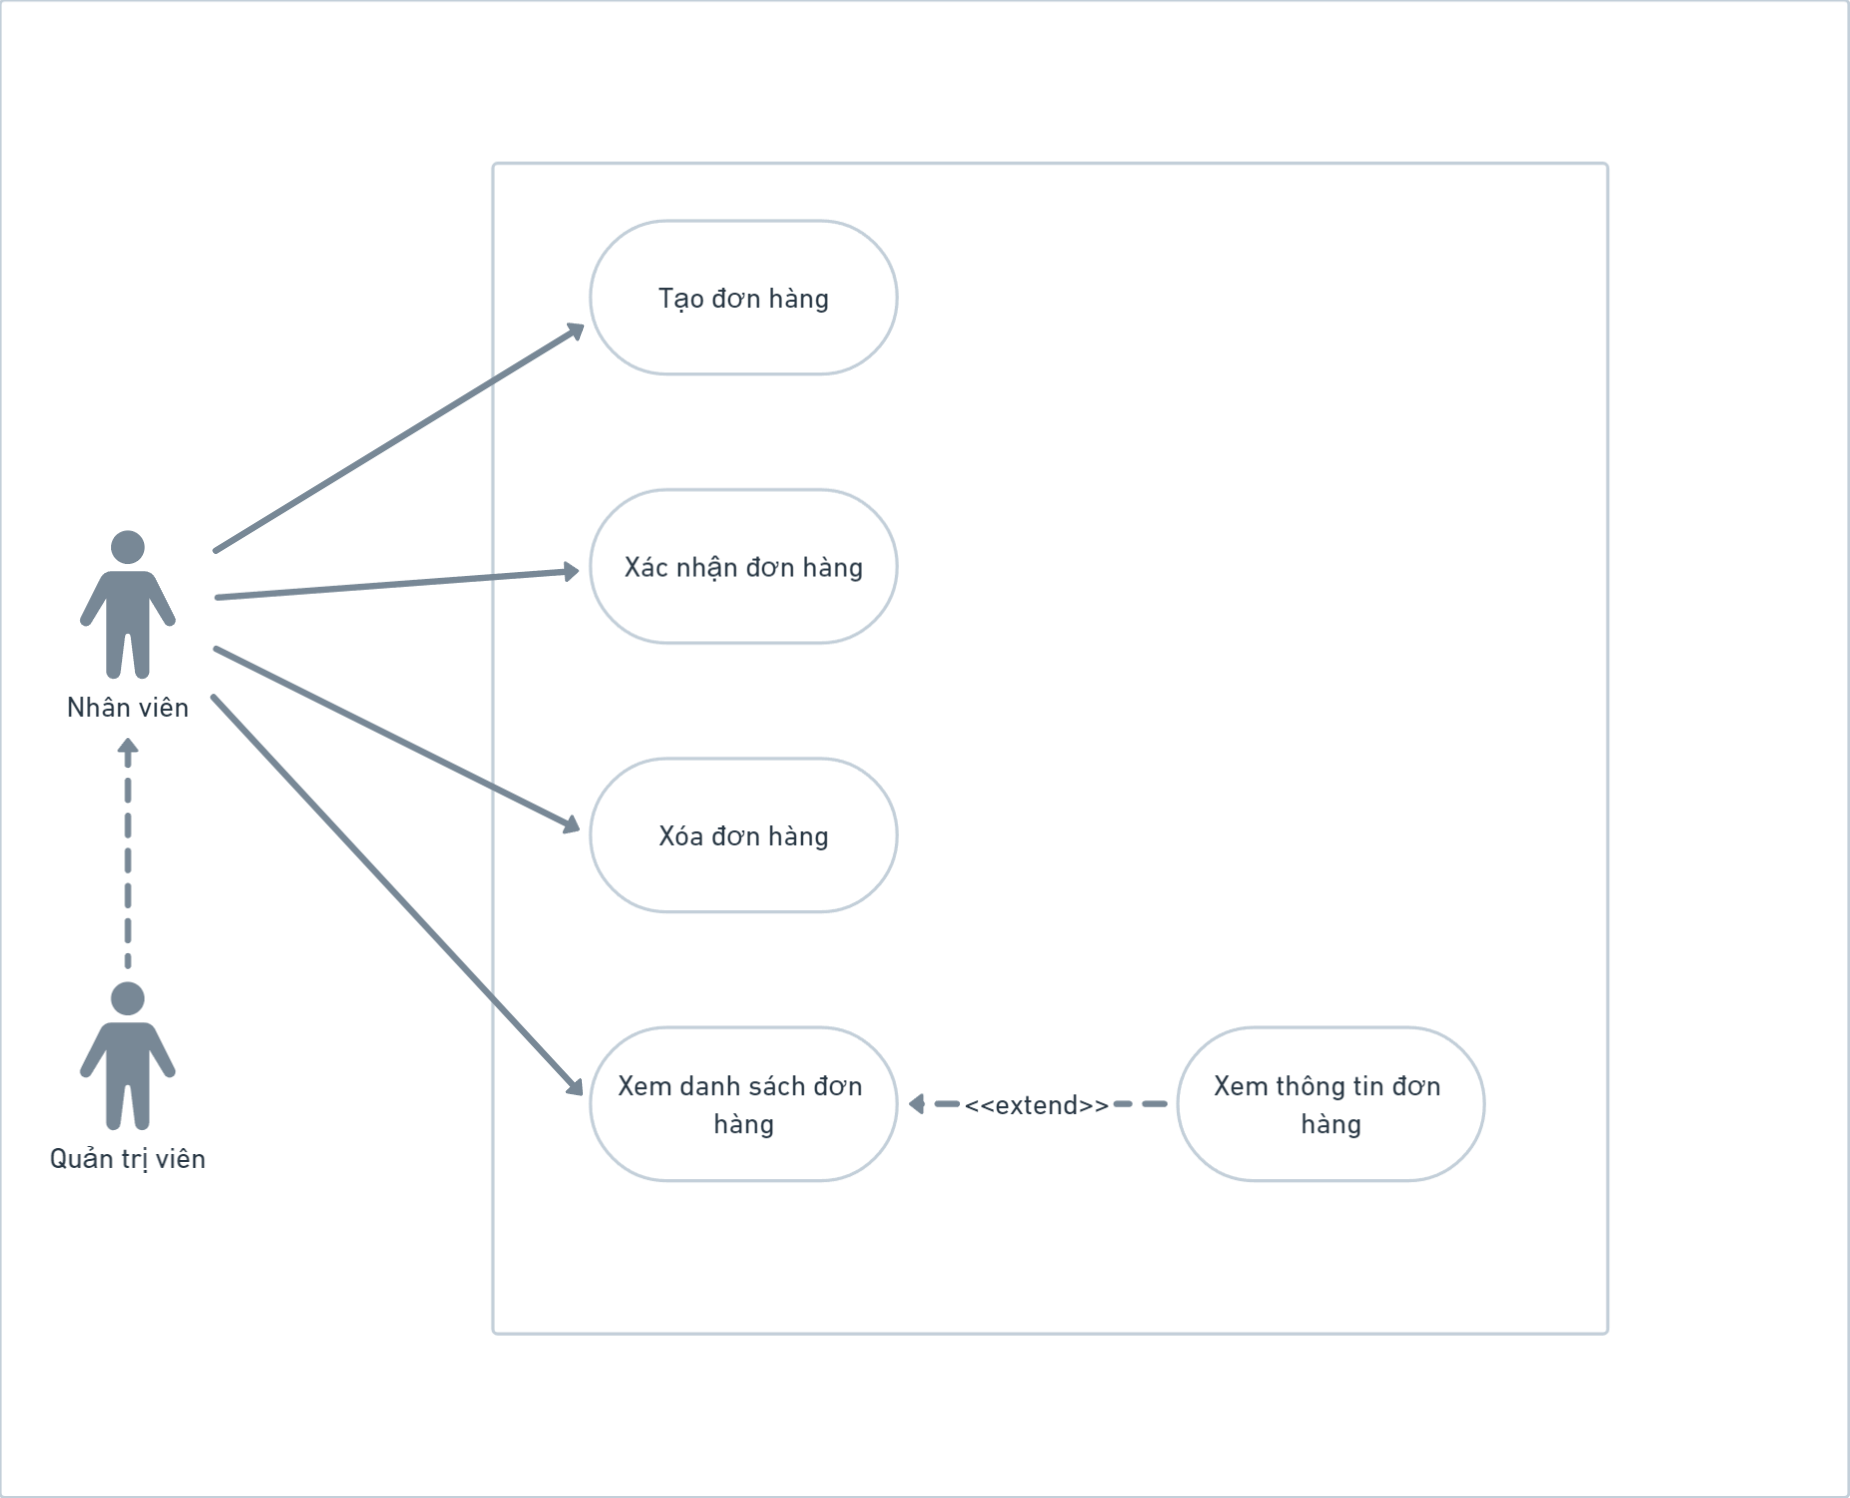
\includegraphics[scale = 0.2]{img/mod/qldh-mod.png}
    \vspace{1cm}
    \caption{Use-case diagram cho module quản lý đơn hàng}
    \label{fig:taskAssignment}
\end{figure}
% \begin{longtable}{|>{\hspace{0pt}}m{0.213\linewidth}|>{\hspace{0pt}}m{0.729\linewidth}|} 
% \hline
% Usecase id & UC2.4.1 \endfirsthead 
% \hline
% Usecase name & Thêm / Xóa / Sửa sản phẩm \\ 
% \hline
% Actor & Nhân viên Quản trị \\ 
% \hline
% Description & Người dùng muốn Thêm, xóa, sửa sản phẩm hiện có trên gian hàng  \\ 
% \hline
% Trigger & Người dùng chọn sản phẩm muốn sửa, xóa hoặc chọn mục "thêm sản phẩm" ở trang dashboard  \\ 
% \hline
% Pre-condition & 1. Có kết nối internet. \\
% & 2. Người dung đã đăng nhập\\ 
% \hline
% Post-condition & 1. Người dùng hoàn thành được tác vụ thêm, xóa, sửa sản phẩm \\ 
% \hline
% Normal Flow & 1. Người dùng chọn sản phẩm.\par{}2. Hệ thống hiện popup có các tùy chọn xóa, sửa sản phẩm \\ 
% \hline
% Alternative Flows & 1a Người dùng chọn thêm sản phẩm\\
% & 1a1. Hệ thống hiện popup thêm sản phẩm vào gian hàng \\
% \hline
% Exceptions & Không \\ 
% \hline
% Business rules & Không \\ 
% \hline
% Non functional-requirement & Không \\ 
% \hline

% \end{longtable}

% \begin{longtable}{|>{\hspace{0pt}}m{0.213\linewidth}|>{\hspace{0pt}}m{0.729\linewidth}|} 
% \hline
% Usecase id & UC2.4.2 \endfirsthead 
% \hline
% Usecase name & Kiểm tra sản phẩm trong kho hàng \\ 
% \hline
% Actor & Nhân viên Quản trị \\ 
% \hline
% Description & Người dùng muốn kiểm tra các sản phẩm trong kho hàng  \\ 
% \hline
% Trigger & Người dùng chọn mục "kho hàng" trên trang dashboard  \\ 
% \hline
% Pre-condition & 1. Có kết nối internet. \\
% & 2. Người dung đã đăng nhập\\ 
% \hline
% Post-condition & 1. Người dùng xem được các sản phẩm còn lại trong kho hàng \\ 
% \hline
% Normal Flow & 1. Người dùng chọn mục "kho hàng" trên trang dashboard.\par{}2. Hệ thống chuyển người dùng tới trang kho hàng \\ 
% \hline
% Alternative Flows & Không \\
% \hline
% Exceptions & Không \\ 
% \hline
% Business rules & Không \\ 
% \hline
% Non functional-requirement & Không \\ 
% \hline

% \end{longtable}

\begin{longtable}{|>{\hspace{0pt}}m{0.213\linewidth}|>{\hspace{0pt}}m{0.729\linewidth}|} 
\hline
Usecase id & UC2.4.1 \endfirsthead 
\hline
Usecase name & Tạo đơn hàng \\ 
\hline
Actor & Nhân viên Quản trị \\ 
\hline
Description & Người dùng muốn tạo đơn hàng mà khác hàng đã đặt  \\ 
\hline
Trigger & Người dùng chọn mục đơn hàng trên thanh dashboard  \\ 
\hline
Pre-condition & 1. Có kết nối internet. \\
& 2. Người dung đã đăng nhập\\ 
\hline
Post-condition & 1. Người dùng tạo được đơn hàng cho khách hàng \\ 
\hline
Normal Flow & 1. Người dùng chọn mục "đơn hàng" trên trang dashboard \par{}2. Hệ thống chuyển người dùng tới trang đơn hàng \par{}3. Người dùng chọn tạo đơn hàng mới \par{}4. Người dùng điền các thông tin cho đơn hàng \par{}5. Người dùng chọn "Tạo đơn hàng" \\  
\hline
Alternative Flows & Không \\
\hline
Exceptions & Không \\ 
\hline
Business rules & Không \\ 
\hline
Non functional-requirement & Không \\ 
\hline
\caption{Use case scenario cho chức năng tạo đơn hàng}
\end{longtable}


\begin{longtable}{|>{\hspace{0pt}}m{0.213\linewidth}|>{\hspace{0pt}}m{0.729\linewidth}|} 
\hline
Usecase id & UC2.4.2 \endfirsthead 
\hline
Usecase name & Xác nhận đơn hàng \\ 
\hline
Actor & Nhân viên Quản trị \\ 
\hline
Description & Người dùng muốn xác nhận đơn hàng mà khác hàng đã đặt  \\ 
\hline
Trigger & Người dùng chọn mục đơn hàng trên thanh dashboard  \\ 
\hline
Pre-condition & 1. Có kết nối internet. \\
& 2. Người dung đã đăng nhập\\ 
\hline
Post-condition & 1. Người dùng xác nhận được đơn hàng \\ 
\hline
Normal Flow & 1. Người dùng chọn mục "đơn hàng" trên trang dashboard \par{}2. Hệ thống chuyển người dùng tới trang đơn hàng \par{}3. Người dùng chọn đơn hàng cụ thể \par{}4. Hệ thống hiện popup chi tiết đơn hàng \par{}5. Người dùng chọn "xác nhận" đơn hàng \\  
\hline
Alternative Flows & Không \\
\hline
Exceptions & Không \\ 
\hline
Business rules & Không \\ 
\hline
Non functional-requirement & Không \\ 
\hline
\caption{Use case scenario cho chức năng xác nhận đơn hàng}

\end{longtable}


\begin{longtable}{|>{\hspace{0pt}}m{0.213\linewidth}|>{\hspace{0pt}}m{0.729\linewidth}|} 
\hline
Usecase id & UC2.4.3 \endfirsthead 
\hline
Usecase name & Xóa đơn hàng \\ 
\hline
Actor & Nhân viên Quản trị \\ 
\hline
Description & Người dùng muốn hủy đơn hàng mà khách hàng đã đặt  \\ 
\hline
Trigger & Người dùng chọn mục đơn hàng trên thanh dashboard  \\ 
\hline
Pre-condition & 1. Có kết nối internet. \\
& 2. Người dung đã đăng nhập\\ 
\hline
Post-condition & 1. Người dùng xác nhận được đơn hàng \\ 
\hline
Normal Flow & 1. Người dùng chọn mục "đơn hàng" trên trang dashboard \par{}2. Hệ thống chuyển người dùng tới trang đơn hàng \par{}3. Người dùng chọn đơn hàng cụ thể \par{}4. Hệ thống hiện popup chi tiết đơn hàng \par{}5. Người dùng chọn "hủy" đơn hàng \\  
\hline
Alternative Flows & Không \\
\hline
Exceptions & Không \\ 
\hline
Business rules & Không \\ 
\hline
Non functional-requirement & Không \\ 
\hline
\caption{Use case scenario cho chức năng xóa đơn hàng}
\end{longtable}

\begin{longtable}{|>{\hspace{0pt}}m{0.213\linewidth}|>{\hspace{0pt}}m{0.729\linewidth}|} 
\hline
Usecase id & UC2.4.4 \endfirsthead 
\hline
Usecase name & Xem thông tin đơn hàng \\ 
\hline
Actor & Nhân viên Quản trị \\ 
\hline
Description & Người dùng muốn kiểm tra thông tin đơn hàng mà khách hàng đã đặt  \\ 
\hline
Trigger & Người dùng chọn mục đơn hàng trên thanh dashboard  \\ 
\hline
Pre-condition & 1. Có kết nối internet. \\
& 2. Người dung đã đăng nhập \par{} 3. Đơn hàng đã được xác nhận\\ 
\hline
Post-condition & 1. Người dùng kiểm tra được thông tin đơn hàng \\ 
\hline
Normal Flow & 1. Người dùng chọn mục "đơn hàng" trên trang dashboard \par{}2. Hệ thống chuyển người dùng tới trang đơn hàng \par{}3. Người dùng chọn đơn hàng cụ thể \par{}4. Hệ thống hiện popup chi tiết đơn hàng \par{}5. Người dùng chọn tùy chọn "thông tin" \par{}6. Hệ thống chuyển người dùng tới trang thông tin đơn hàng \\  
\hline
Alternative Flows & Không \\
\hline
Exceptions & Không \\ 
\hline
Business rules & Không \\ 
\hline
Non functional-requirement & Không \\ 
\hline
\caption{Use case scenario cho chức năng xem thông tin đơn hàng}
\end{longtable}

% \begin{longtable}{|>{\hspace{0pt}}m{0.213\linewidth}|>{\hspace{0pt}}m{0.729\linewidth}|} 
% \hline
% Usecase id & UC2.4.6 \endfirsthead 
% \hline
% Usecase name & Tạo mã giảm giá \\ 
% \hline
% Actor & Nhân viên Quản trị \\ 
% \hline
% Description & Người dùng muốn tạo mã giảm giá cho các sản phẩm cụ thể  \\ 
% \hline
% Trigger & Người dùng chọn mục mã giảm giá trên thanh dashboard  \\ 
% \hline
% Pre-condition & 1. Có kết nối internet. \\
% & 2. Người dung đã đăng nhập\\ 
% \hline
% Post-condition & 1.Người dùng tạo được mã giảm giá \\ 
% \hline
% Normal Flow & 1. Người dùng chọn mục "mã giảm giá" trên trang dashboard \par{}2. Hệ thống chuyển người dùng tới trang mã giảm giá \par{}3. Người dùng chọn "tạo mã giảm giá" \par{}4. Hệ thống hiện popup chi tiết điều kiện mã giảm giá được áp dụng \par{}5. Người dùng chọn tùy chọn "Tạo mã" \par{}6. Hệ thống tạo mã thành công \\  
% \hline
% Alternative Flows & Không \\
% \hline
% Exceptions & Không \\ 
% \hline
% Business rules & Không \\ 
% \hline
% Non functional-requirement & Không \\ 
% \hline
% \end{longtable}

\newpage
\subsection{Module quản lý sản phẩm}
\begin{figure}[h]
    \centering
    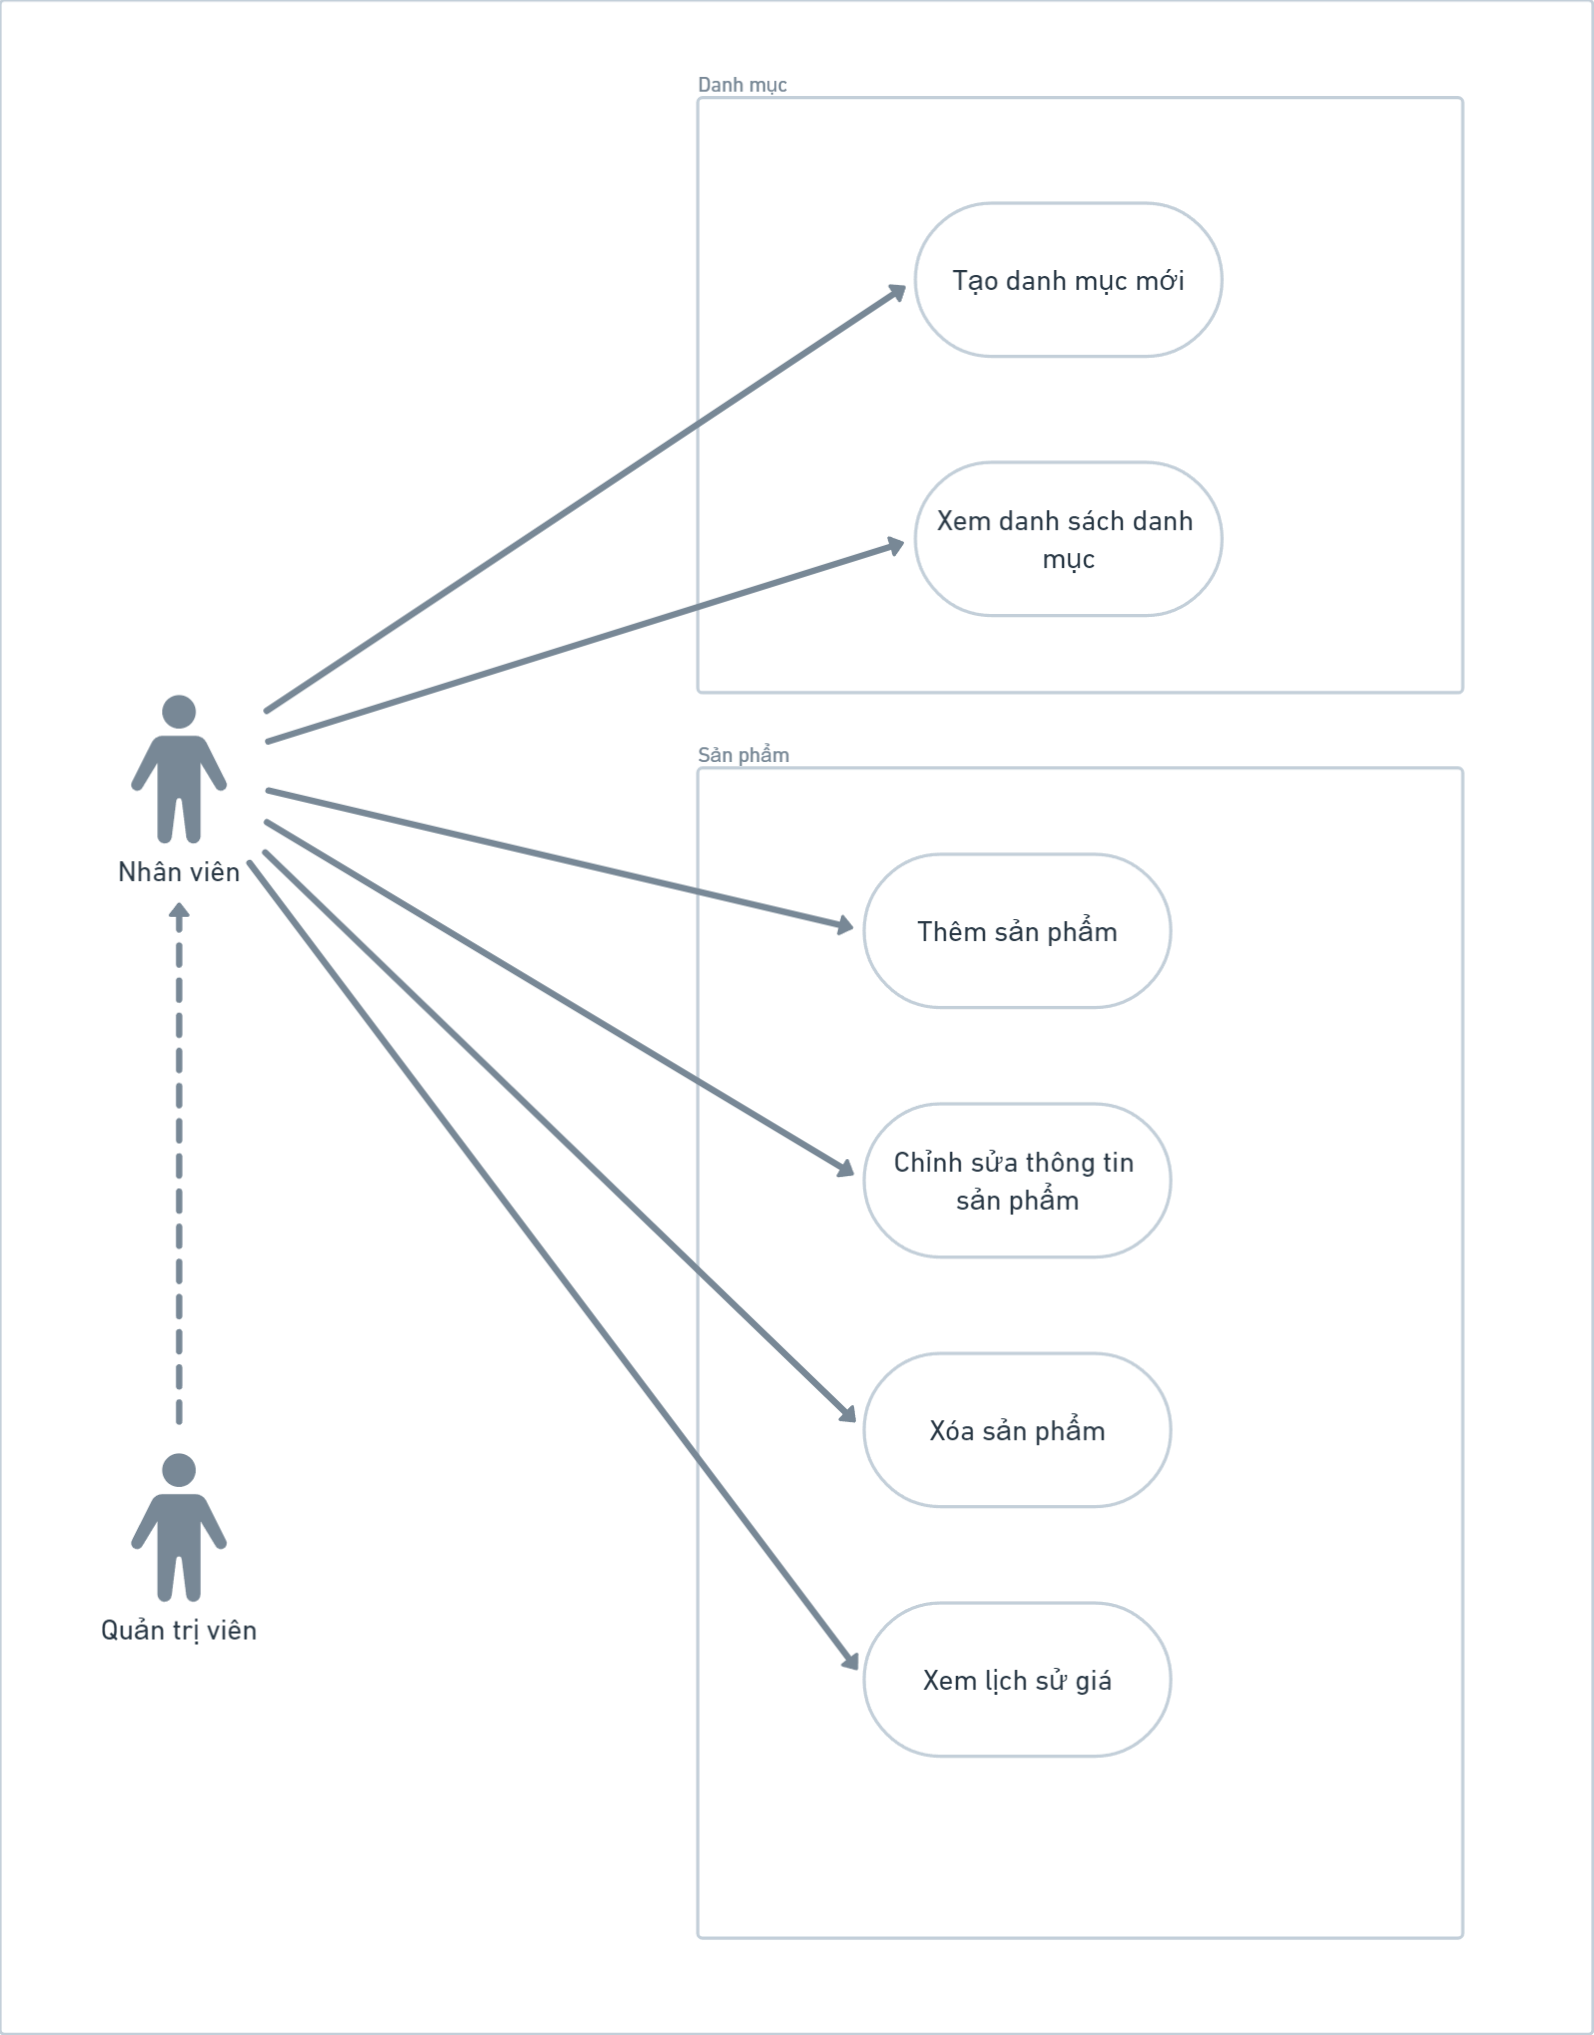
\includegraphics[scale = 0.2]{img/mod/qlsp-mod.png}
    \vspace{1cm}
    \caption{Use-case diagram cho module quản lý sản phẩm}
    \label{fig:taskAssignment}
\end{figure}

\begin{longtable}{|>{\hspace{0pt}}m{0.213\linewidth}|>{\hspace{0pt}}m{0.729\linewidth}|} 
\hline
Usecase id & UC2.5.1 \endfirsthead 
\hline
Usecase name & Thêm / Xóa / Sửa sản phẩm \\ 
\hline
Actor & Nhân viên Quản trị \\ 
\hline
Description & Người dùng muốn Thêm, xóa, sửa sản phẩm hiện có trên gian hàng  \\ 
\hline
Trigger & Người dùng chọn sản phẩm muốn sửa, xóa hoặc chọn mục "thêm sản phẩm" ở trang dashboard  \\ 
\hline
Pre-condition & 1. Có kết nối internet. \\
& 2. Người dung đã đăng nhập\\ 
\hline
Post-condition & 1. Người dùng hoàn thành được tác vụ thêm, xóa, sửa sản phẩm \\ 
\hline
Normal Flow & 1. Người dùng chọn sản phẩm.\par{}2. Hệ thống hiện popup có các tùy chọn xóa, sửa sản phẩm \\ 
\hline
Alternative Flows & 1a Người dùng chọn thêm sản phẩm\\
& 1a1. Hệ thống hiện popup thêm sản phẩm vào gian hàng \\
\hline
Exceptions & Không \\ 
\hline
Business rules & Không \\ 
\hline
Non functional-requirement & Không \\ 
\hline
\caption{Use case scenario cho chức năng Thêm / Xóa / Sửa sản phẩm}

\end{longtable}

%%%%%

\newpage
\subsection{Module tương tác sản phẩm}
\begin{figure}[h]
    \centering
    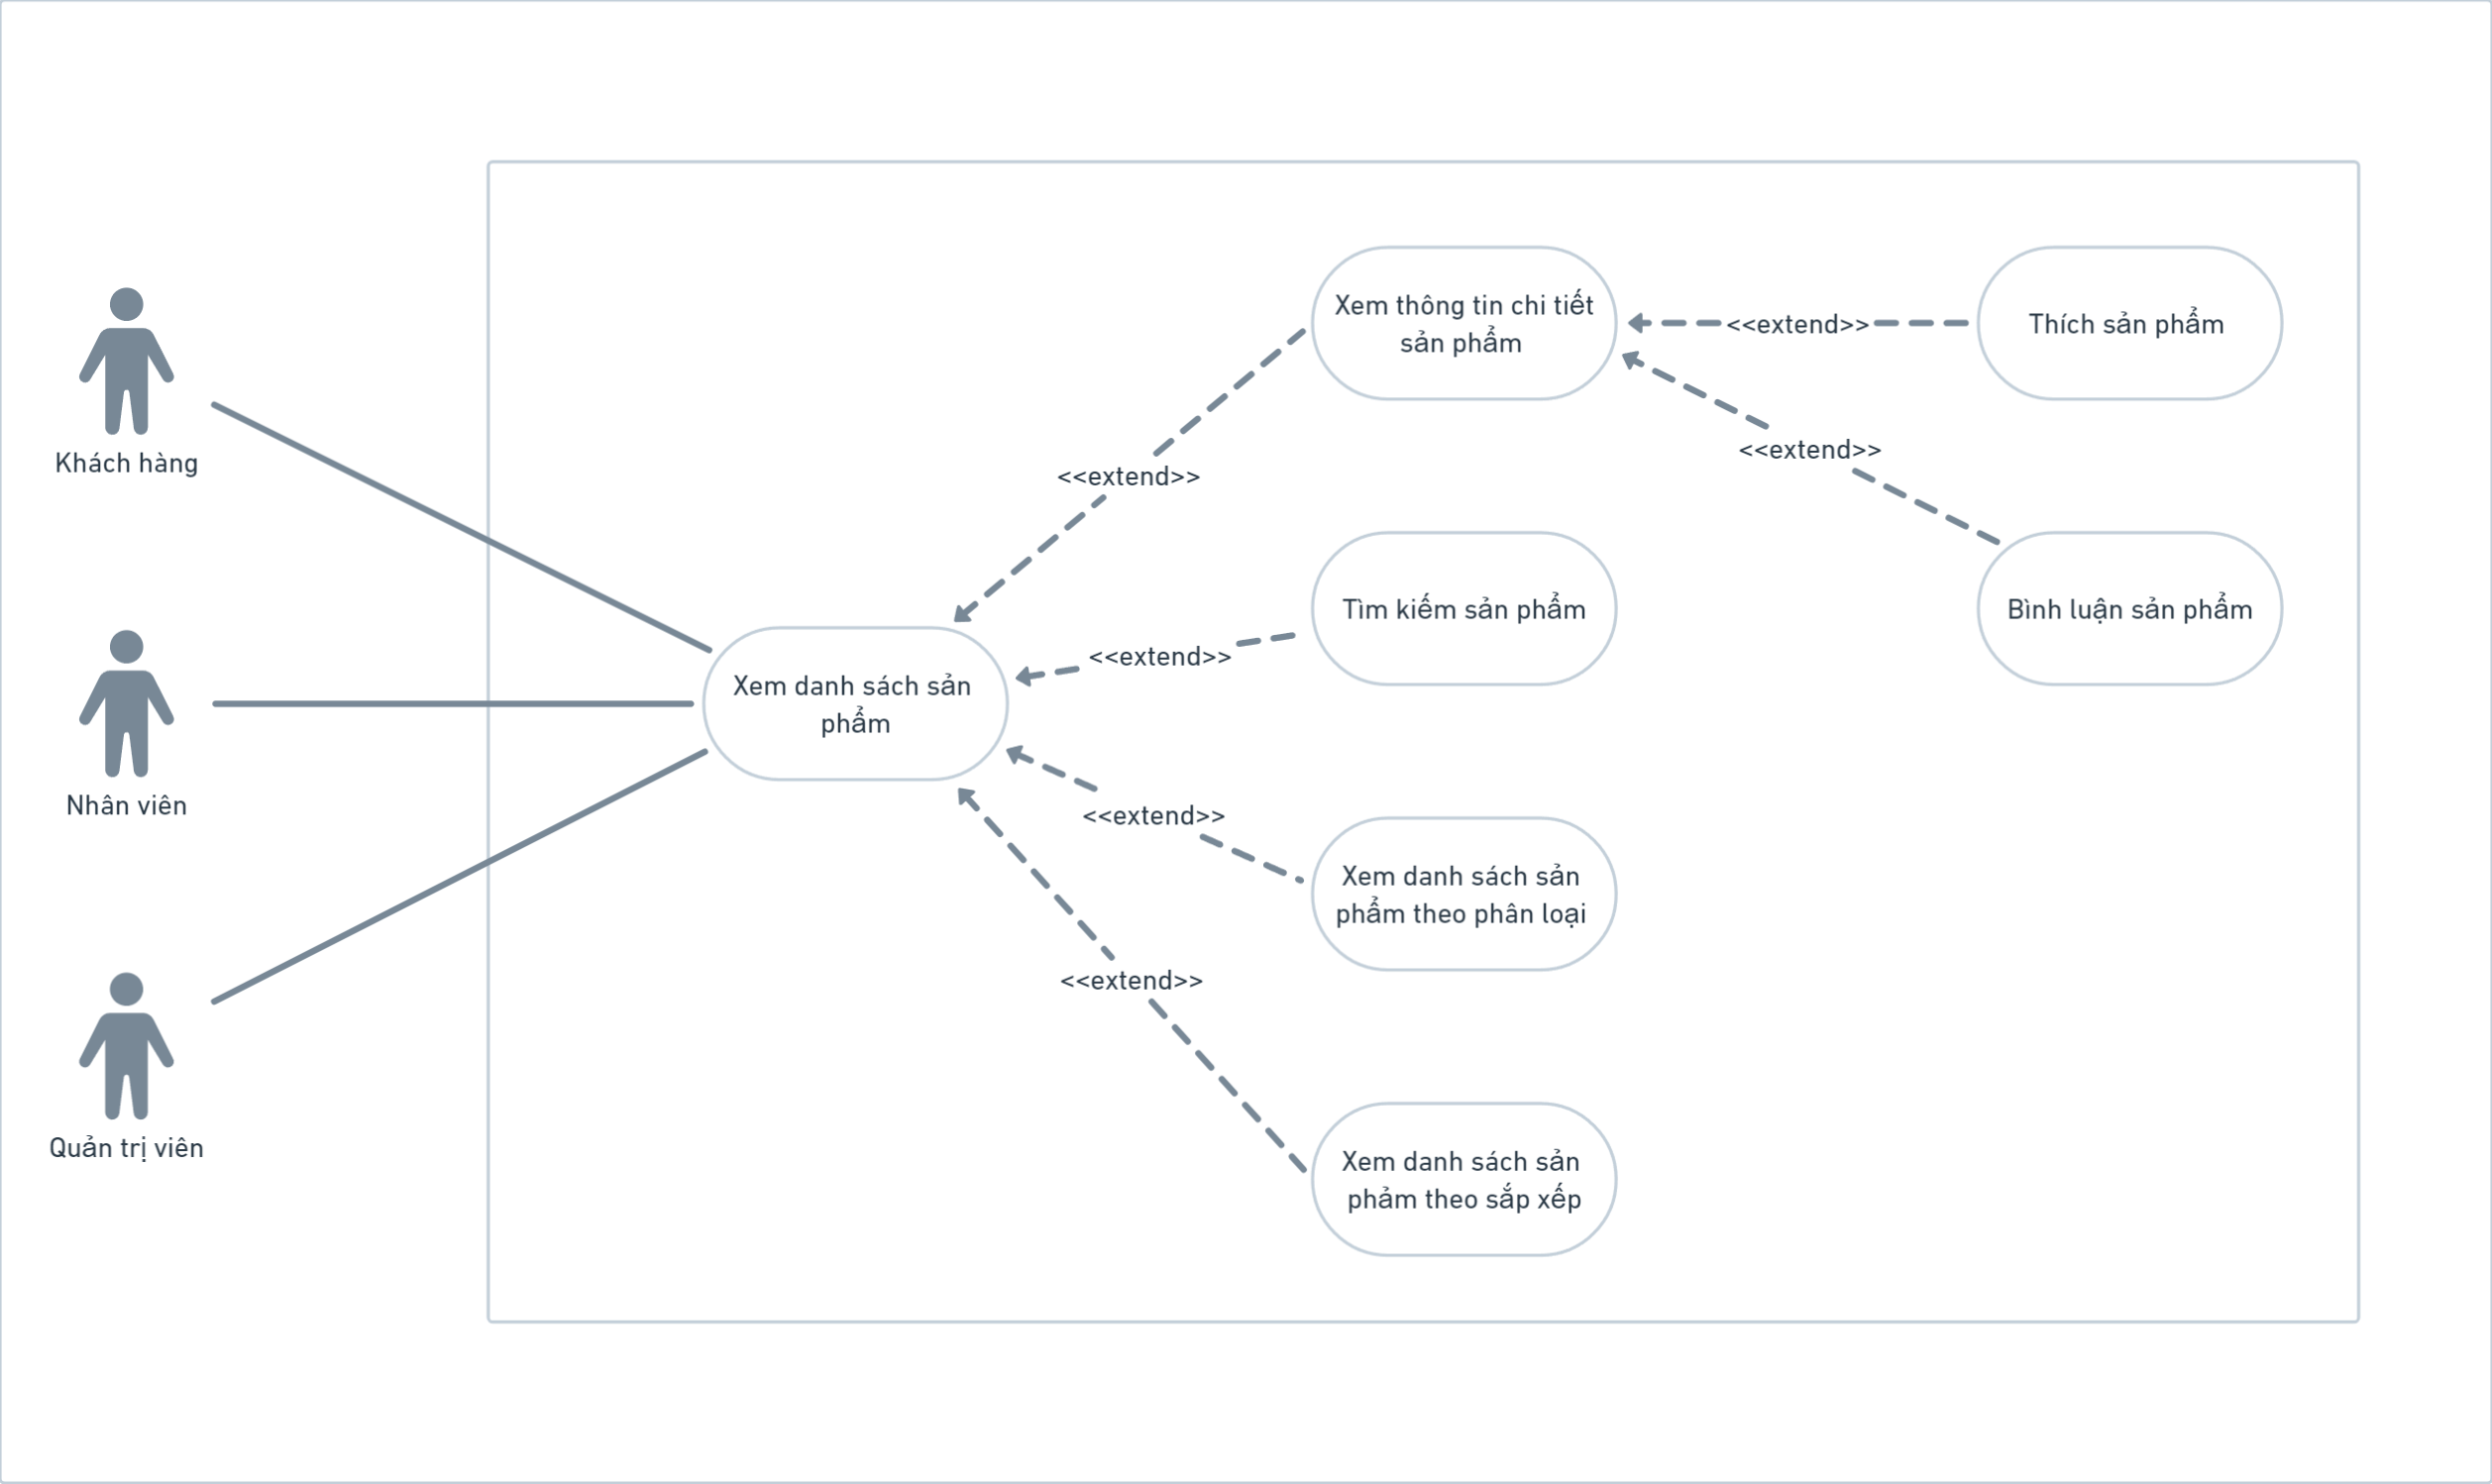
\includegraphics[scale = 0.2]{img/mod/ttsp-mod.png}
    \vspace{0.5cm}
    \caption{Use-case diagram cho module tương tác sản phẩm}
    \label{fig:taskAssignment}
\end{figure}

% \usepackage{array}
% \usepackage{longtable}

\begin{longtable}{|>{\hspace{0pt}}m{0.229\linewidth}|>{\hspace{0pt}}m{0.713\linewidth}|} 
\hline
Usecase id & UC2.6.1 \endfirsthead 
\hline
Usecase name & Xem danh sách sản phẩm \\ 
\hline
Actor & Khách hàng, nhân viên, quản trị viên \\ 
\hline
Description & Người dùng muốn xem danh sách các sản phẩm \\ 
\hline
Trigger & Người dùng nhấn vào Danh sách sản phẩm \\ 
\hline
Pre-condition & 1. Có kết nối internet.\par{}2. Người dùng đã đăng nhập thành công. \\ 
\hline
Post-condition & 1. Người dùng xem được danh sách các sản phẩm \\
\hline
Normal Flow & 1. Người dùng nhấn vào Danh sách sản phẩm.\par{}2. Hệ thống chuyển người dùng đến trang hiển thị các sản phẩm người dùng mong muốn.\par{}2.1 Người dùng nhấn vào sản phẩm muốn xem để xem chi tiết sản phẩm.\\
\hline
Alternative Flows & Không~ \\ 
\hline
Exceptions & Không \\ 
\hline
Business rules & Không \\ 
\hline
Non functional-requirement & Không \\ 
\hline
\caption{Use case scenario cho chức năng Xem danh sách sản phẩm}

\end{longtable}

% \usepackage{array}
% \usepackage{longtable}

\begin{longtable}{|>{\hspace{0pt}}m{0.213\linewidth}|>{\hspace{0pt}}m{0.729\linewidth}|} 
\hline
Usecase id & UC2.6.2 \endfirsthead 
\hline
Usecase name & Xem Chi tiết sản phẩm \\ 
\hline
Actor & Khách hàng, nhân viên, quản trị viên \\ 
\hline
Description & Người dùng muốn xem chi tiết sản phẩm \\ 
\hline
Trigger & Người dùng nhấn vào sản phẩm \\ 
\hline
Pre-condition & 1. Có kết nối internet. \\ 
\hline
Post-condition & 1. Người dùng xem được chi tiết sản phẩm \\ 
\hline
Normal Flow & 1. Người dùng nhấn vào mục sản phẩm cụ thể.\par{}2. Hệ thống chuyển người dùng đến trang chi tiết sản phẩm \\ 
\hline
Alternative Flows & Không~ \\ 
\hline
Exceptions & Không \\ 
\hline
Business rules & Không \\ 
\hline
Non functional-requirement & Không \\ 
\hline
\caption{Use case scenario cho chức năng Xem Chi tiết sản phẩm}

\end{longtable}

% \usepackage{array}
% \usepackage{longtable}

\begin{longtable}{|>{\hspace{0pt}}m{0.213\linewidth}|>{\hspace{0pt}}m{0.729\linewidth}|} 
\hline
Usecase id & UC2.6.3 \endfirsthead 
\hline
Usecase name & Tìm kiếm sản phẩm \\ 
\hline
Actor & Khách hàng, nhân viên, quản trị viên \\ 
\hline
Description & Người dùng muốn tìm kiếm sản phẩm theo từ khóa\\ 
\hline
Trigger & Người dùng nhấn vào ô tìm kiếm sản phẩm \\ 
\hline
Pre-condition & 1. Có kết nối internet. \\ 
\hline
Post-condition & 1. Người dùng tìm được sản phẩm mình muốn theo từ khóa \\ 
\hline
Normal Flow & 1. Người dùng truy cập vào trang chủ hoặc trang danh sách sản phẩm.\par{}2. Người dùng nhập vào từ khóa sản phẩm muốn tìm vào ô tìm kiếm.\par{}3. Hệ thống sẽ trả ra các sản phẩm liên quan. \\ 
\hline
Alternative Flows & Không~ \\ 
\hline
Exceptions & Hệ thống bảo trì tạm thời \\ 
\hline
Business rules & Không \\ 
\hline
Non functional-requirement & Không \\                                   
\hline
\caption{Use case scenario cho chức năng Tìm kiếm sản phẩm}

\end{longtable}

% \usepackage{array}
% \usepackage{longtable}

\begin{longtable}{|>{\hspace{0pt}}m{0.213\linewidth}|>{\hspace{0pt}}m{0.729\linewidth}|} 
\hline
Usecase id & UC2.6.4 \endfirsthead 
\hline
Usecase name & Thích sản phẩm \\ 
\hline
Actor & Khách hàng, nhân viên, quản trị viên \\ 
\hline
Description & Người dùng muốn thêm sản phẩm vào yêu thích\\ 
\hline
Trigger & Người dùng nhấn vào biểu tượng thêm sản phẩm vào yêu thích \\ 
\hline
Pre-condition & 1. Có kết nối internet. \\ 
\hline
Post-condition & 1. Người dùng thêm sản phầm mình yêu thích vào danh sách yêu thích \\ 
\hline
Normal Flow & 1. Người dùng truy cập vào trang chủ.\par{}2. Người dùng nhập thấy sản phẩm mình yêu thích và bấm thích sản phẩm.\par{}3. Hệ thống sẽ đưa sản phẩm người dùng thích vào danh sách yêu thích. \\ 
\hline
Alternative Flows & 1.1. Người dùng truy cập vào danh sách sản phẩm.\par{} 1.2 Người dùng truy cập vào trang chi tiết sản phẩm \\ 
\hline
Exceptions & Hệ thống bảo trì tạm thời \\ 
\hline
Business rules & Không \\ 
\hline
Non functional-requirement & Không \\ 
\hline
\caption{Use case scenario cho chức năng Thích sản phẩm}
\end{longtable}

% \usepackage{array}
% \usepackage{longtable}

\begin{longtable}{|>{\hspace{0pt}}m{0.229\linewidth}|>{\hspace{0pt}}m{0.713\linewidth}|} 
\hline
Usecase id & UC2.6.5 \endfirsthead 
\hline
Usecase name & Xem danh sách sản phẩm theo phân loại \\ 
\hline
Actor & Khách hàng, nhân viên, quản trị viên \\ 
\hline
Description & Người dùng muốn xem danh sách các sản phẩm theo phân loại sản phẩm\\ 
\hline
Trigger & Người dùng nhấn vào Danh sách sản phẩm và chọn phân loại muốn xem  \\ 
\hline
Pre-condition & 1. Có kết nối internet.\par{}2. Người dùng đã đăng nhập thành công. \\ 
\hline
Post-condition & 1. Người dùng xem được danh sách các sản phẩm theo phân loại\\
\hline
Normal Flow & 1. Người dùng nhấn vào Danh sách sản phẩm.\par{}2. Hệ thống chuyển người dùng đến trang hiển thị các sản phẩm.\par{}2.1 Người dùng nhấn vào phân loại các sản phẩm muốn xem.\par{} 4. Hệ thống hiện danh sách các sản phẩm theo phân loại người dùng chọn. \\
\hline
Alternative Flows & Không~ \\ 
\hline
Exceptions & Không \\ 
\hline
Business rules & Không \\ 
\hline
Non functional-requirement & Không \\ 
\hline
\caption{Use case scenario cho chức năng Xem danh sách sản phẩm theo phân loại}
\end{longtable}

% \usepackage{array}
% \usepackage{longtable}

\begin{longtable}{|>{\hspace{0pt}}m{0.229\linewidth}|>{\hspace{0pt}}m{0.713\linewidth}|} 
\hline
Usecase id & UC2.6.6 \endfirsthead 
\hline
Usecase name & Xem danh sách sản phẩm theo sắp xếp \\ 
\hline
Actor & Khách hàng, nhân viên, quản trị viên \\ 
\hline
Description & Người dùng muốn xem danh sách các sản phẩm theo sắp xếp\\ 
\hline
Trigger & Người dùng nhấn vào Danh sách sản phẩm và chọn sắp xếp  \\ 
\hline
Pre-condition & 1. Có kết nối internet.\par{}2. Người dùng đã đăng nhập thành công. \\ 
\hline
Post-condition & 1. Người dùng xem được danh sách các sản phẩm theo sắp xếp mong muốn \\
\hline
Normal Flow & 1. Người dùng nhấn vào Danh sách sản phẩm.\par{}2 Người dùng nhấn vào sắp xếp sản phẩm theo mong muốn.\par{} 3. Hệ thống hiện danh sách các sản phẩm đã được sắp xếp. \\
\hline
Alternative Flows & Không~ \\ 
\hline
Exceptions & Không \\ 
\hline
Business rules & Không \\ 
\hline
Non functional-requirement & Không \\ 
\hline
\caption{Use case scenario cho chức năng Xem danh sách sản phẩm theo sắp xếp}

\end{longtable}

\newpage
\subsection{Module chăm sóc khách hàng}
\begin{figure}[h]
    \centering
    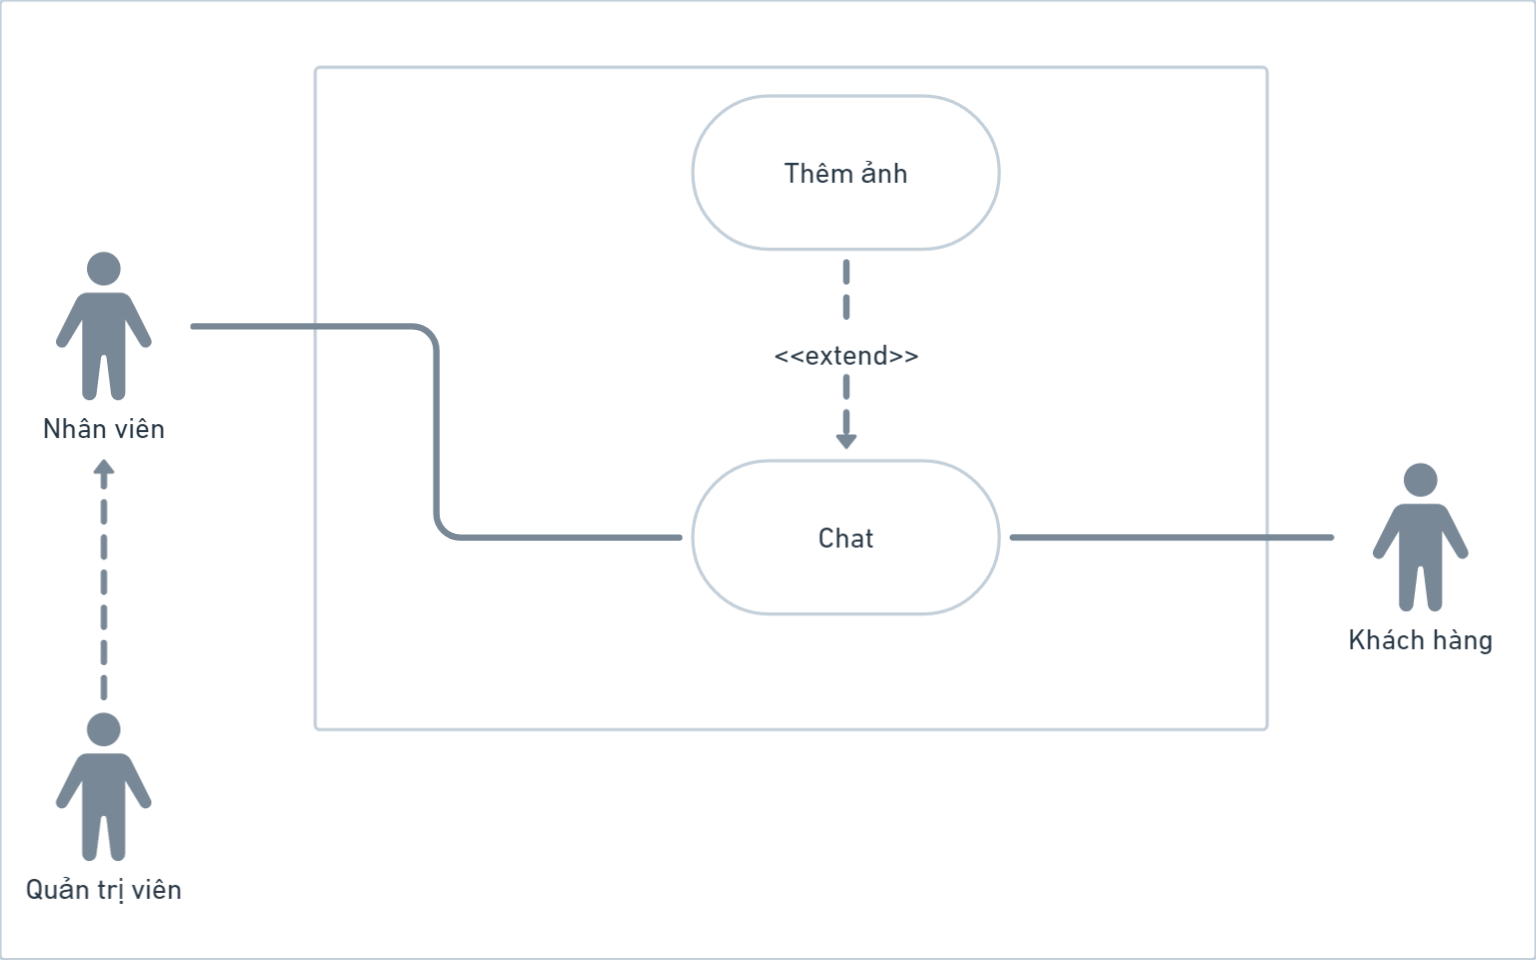
\includegraphics[scale = 0.2]{img/mod/chatcskh.png}
    \vspace{1cm}
    \caption{Use-case diagram cho module chăm sóc khách hàng}
    \label{fig:taskAssignment}
\end{figure}

\begin{longtable}{|>{\hspace{0pt}}m{0.213\linewidth}|>{\hspace{0pt}}m{0.729\linewidth}|} 
\hline
Usecase id & UC2.7.1 \endfirsthead 
\hline
Usecase name & Trò chuyện với bộ phận chăm sóc khách hàng \\ 
\hline
Actor & Khách hàng \\ 
\hline
Description & Người dùng muốn trao đổi với nhân viên chăm sóc khách hàng \\ 
\hline
Trigger & Người dùng chọn mục trò chuyện ở trang chủ  \\ 
\hline
Pre-condition & 1. Có kết nối internet. \\
& 2. Người dung đã đăng nhập\\ 
\hline
Post-condition & 1. Người dùng trò chuyện trực tiếp với nhân viên \\ 
\hline
Normal Flow & 1. Người dùng chọn mục trò chuyện với nhân viên.\par{}2. Hệ thống kết nối người dùng trực tiếp với nhân viên đang hoạt động \\ 
\hline
Alternative Flows & Không\\
\hline
Exceptions & Không \\ 
\hline
Business rules & Không \\ 
\hline
Non functional-requirement & Không \\ 
\hline
\caption{Use case scenario cho chức năng Trò chuyện với bộ phận chăm sóc khách hàng}
\end{longtable}

\newpage
\section{Sequence diagram}
\newpage
\section{Activity diagram - Luồng hoạt động của hệ thống}
\subsection{Đăng nhập, đăng kí}
\begin{figure}[h]
    \centering
    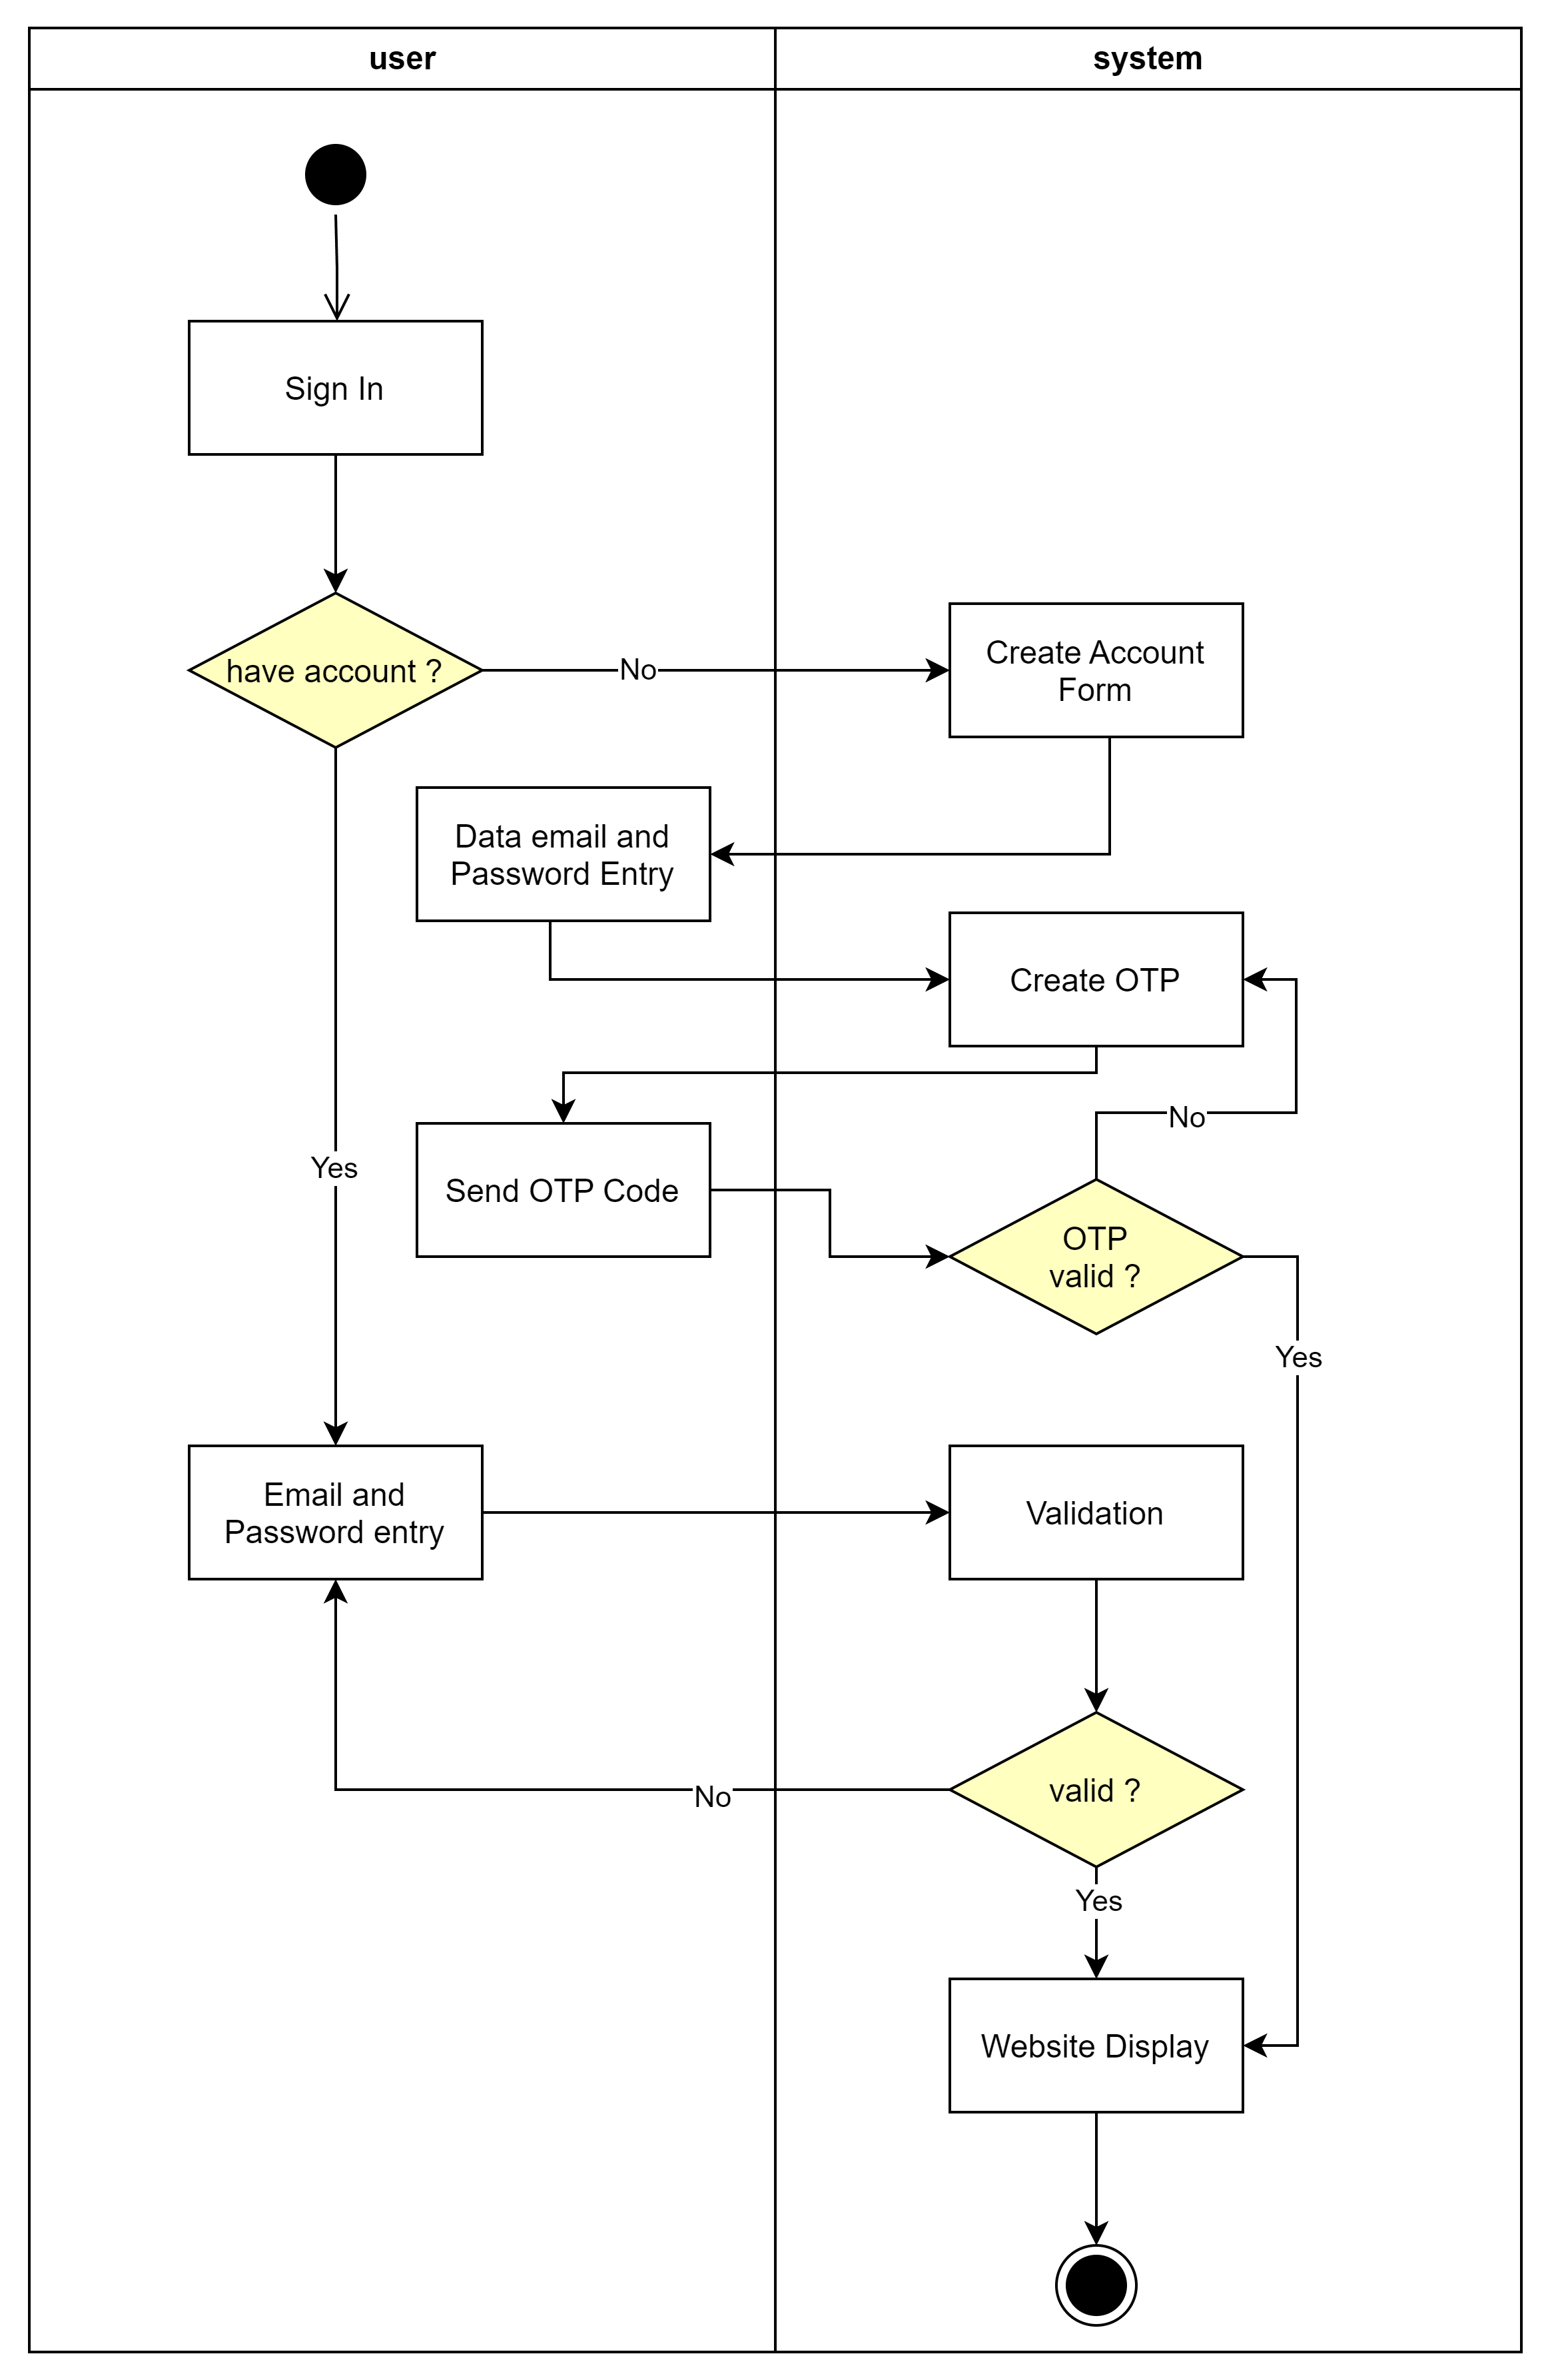
\includegraphics[scale = 0.13]{img/activity/signin.png}
    \vspace{1cm}
    \caption{Activity diagram cho chức năng đăng nhập, đăng kí tài khoản}
    \label{fig:taskAssignment}
\end{figure}

\newpage
\subsection{Đặt hàng, thanh toán}
\begin{figure}[h]
    \centering
    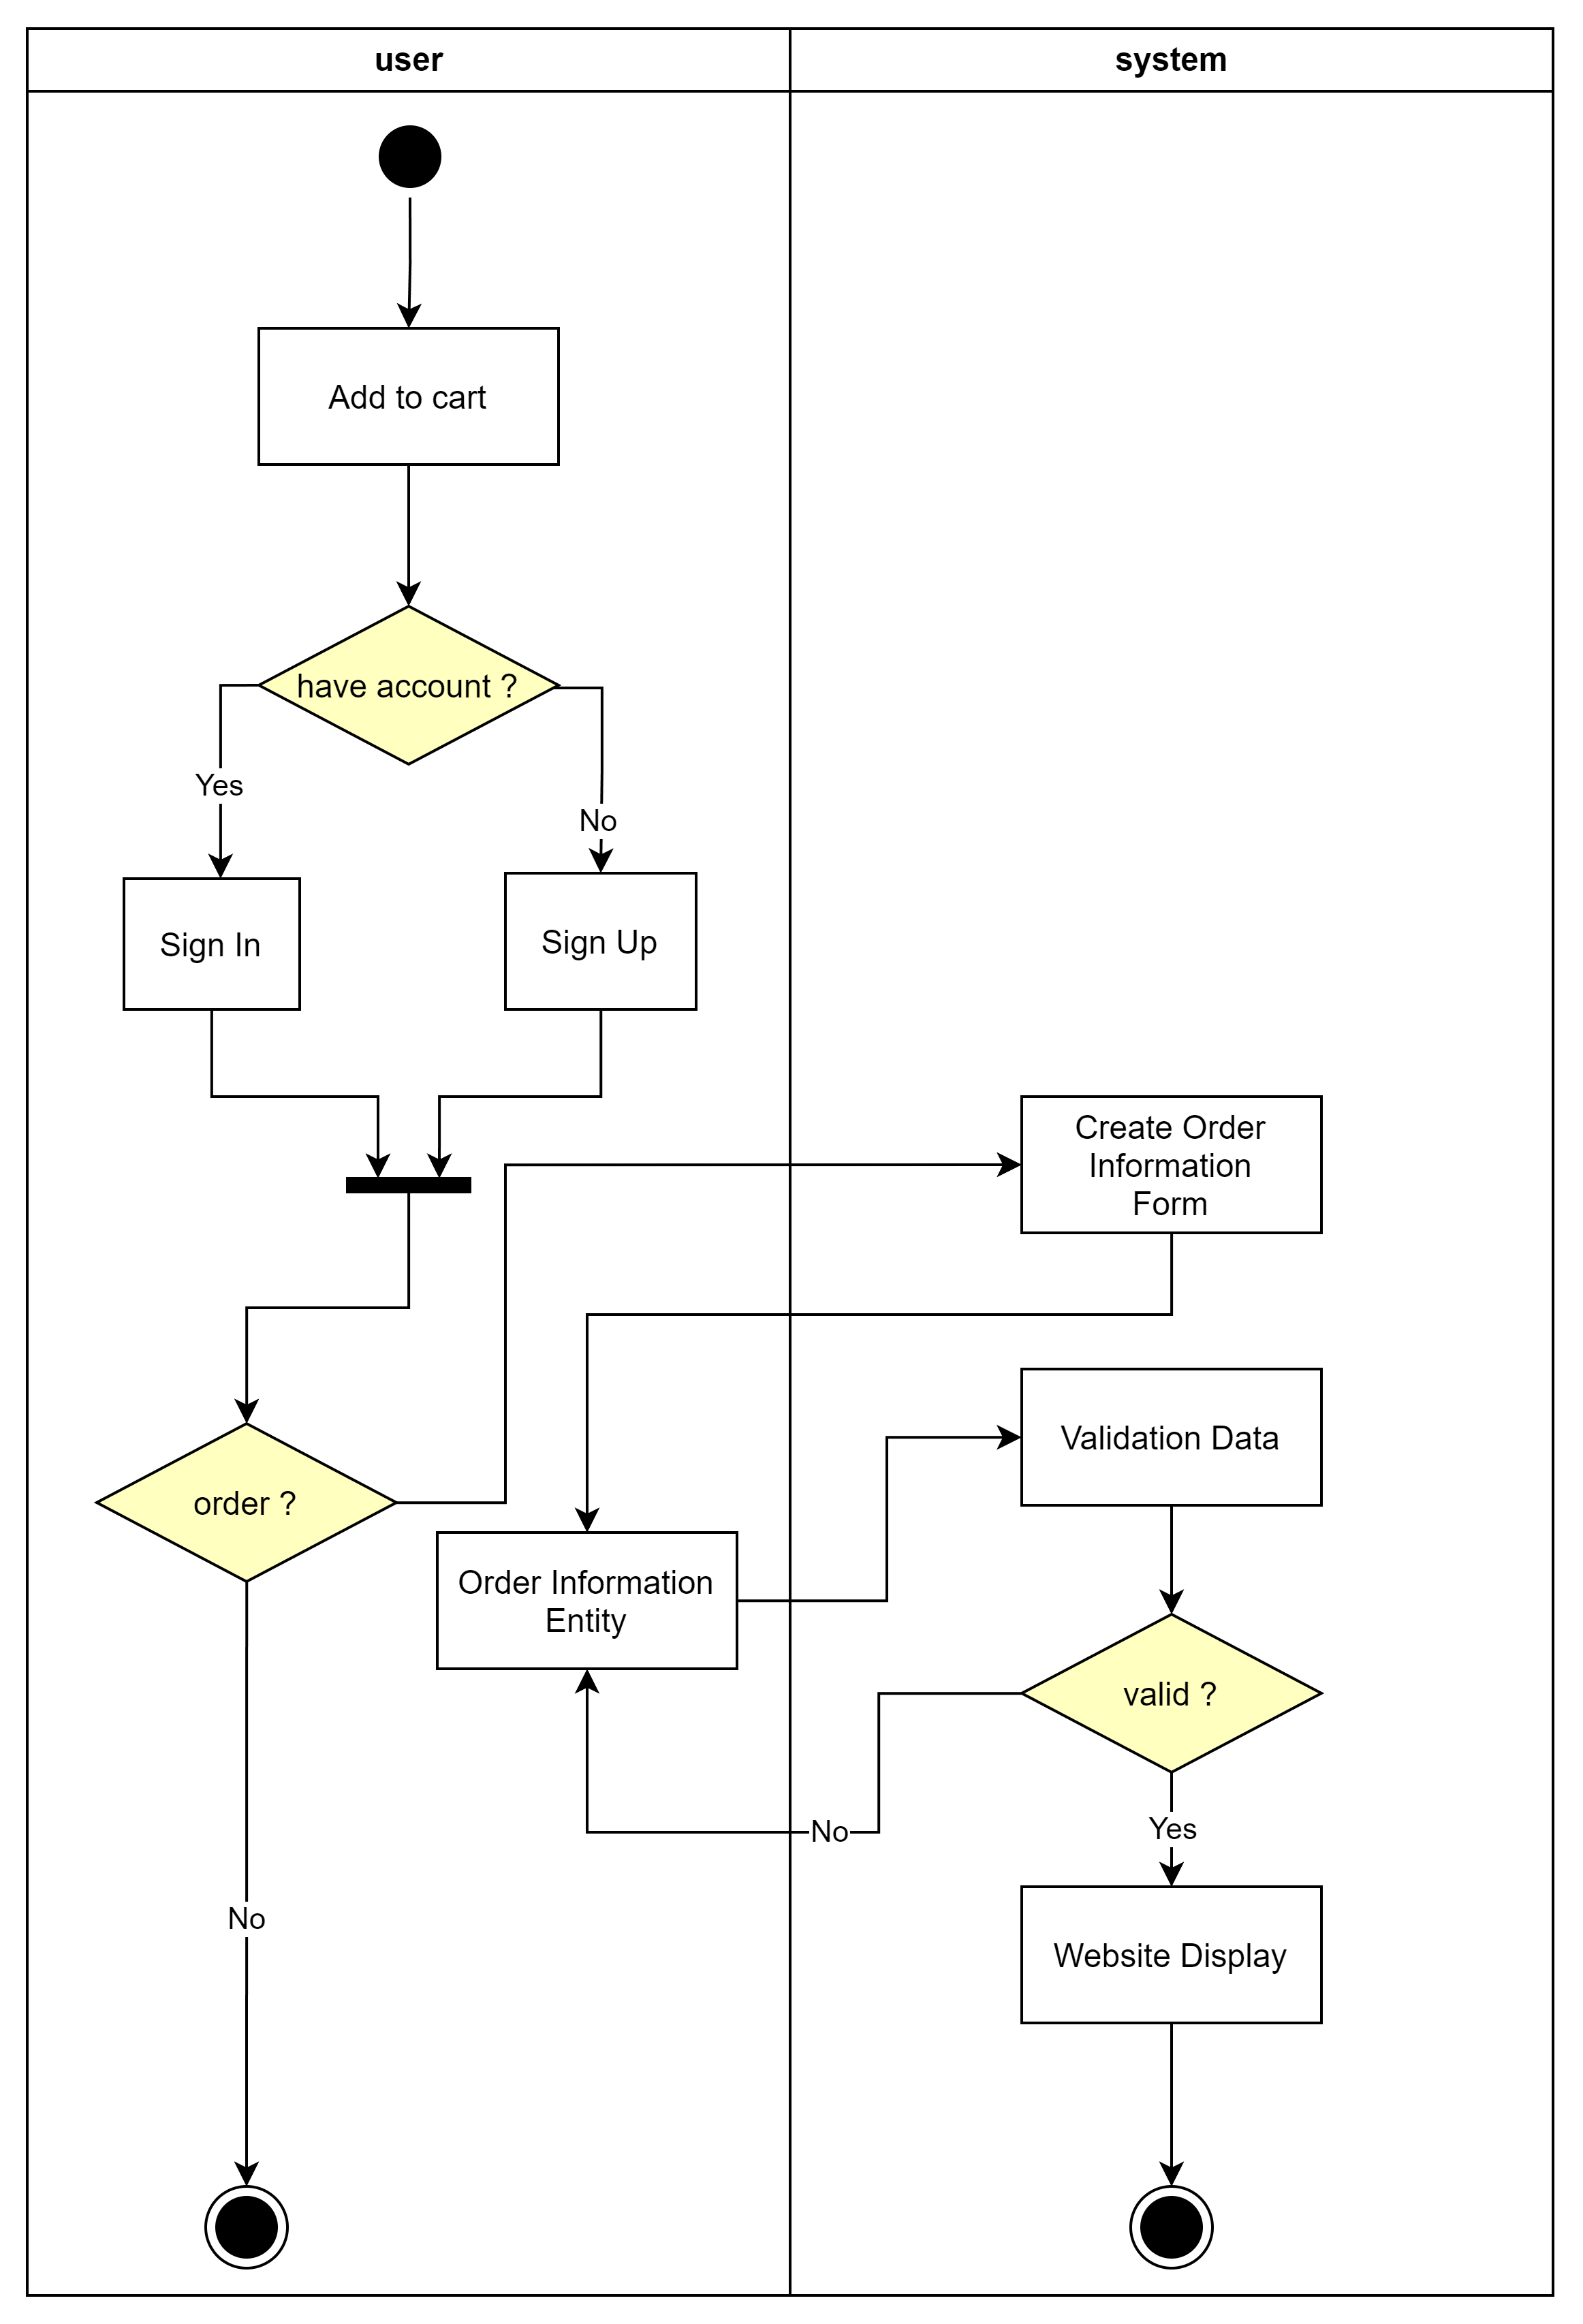
\includegraphics[scale = 0.12]{img/activity/order.png}
    \vspace{1cm}
    \caption{Activity diagram cho chức năng đặt hàng}
    \label{fig:taskAssignment}
\end{figure}

\newpage
\begin{figure}[h]
    \centering
    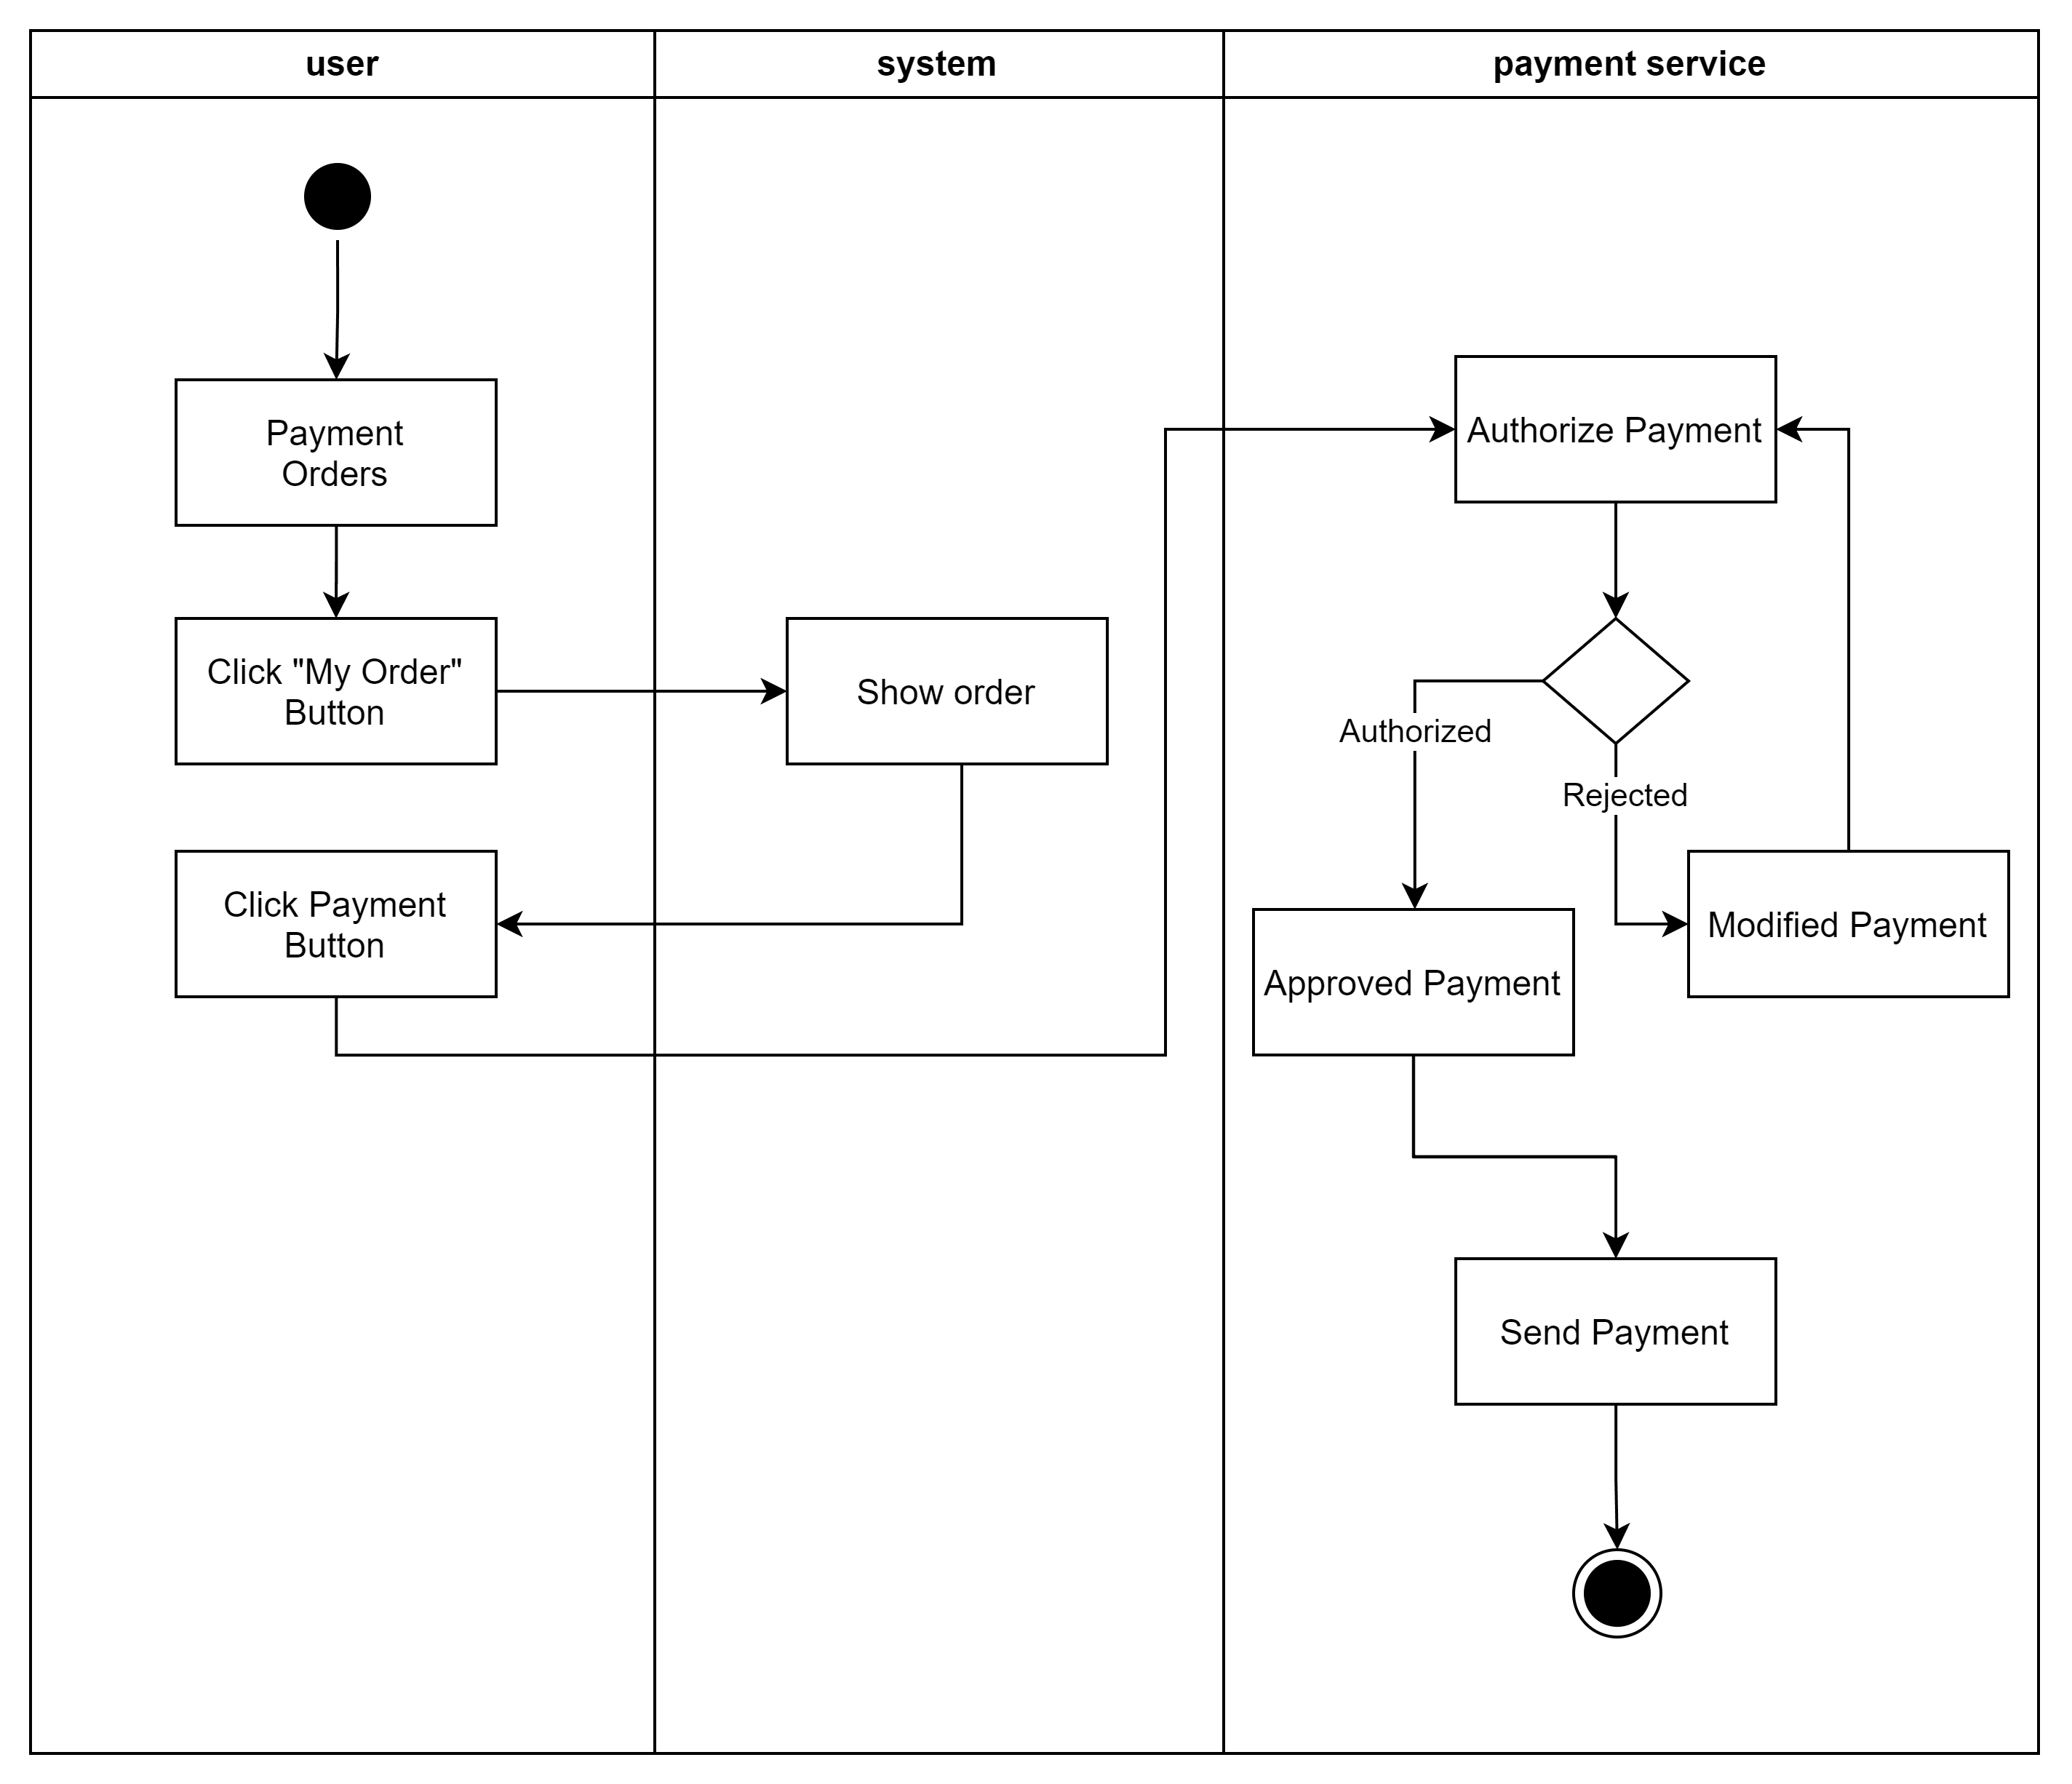
\includegraphics[scale = 0.15]{img/activity/payment.png}
    \vspace{1cm}
    \caption{Activity diagram cho chức năng thanh toán}
    \label{fig:taskAssignment}
\end{figure}

\newpage
\subsection{Thêm sản phẩm yêu thích, bình luận bài viết}
\begin{figure}[h]
    \centering
    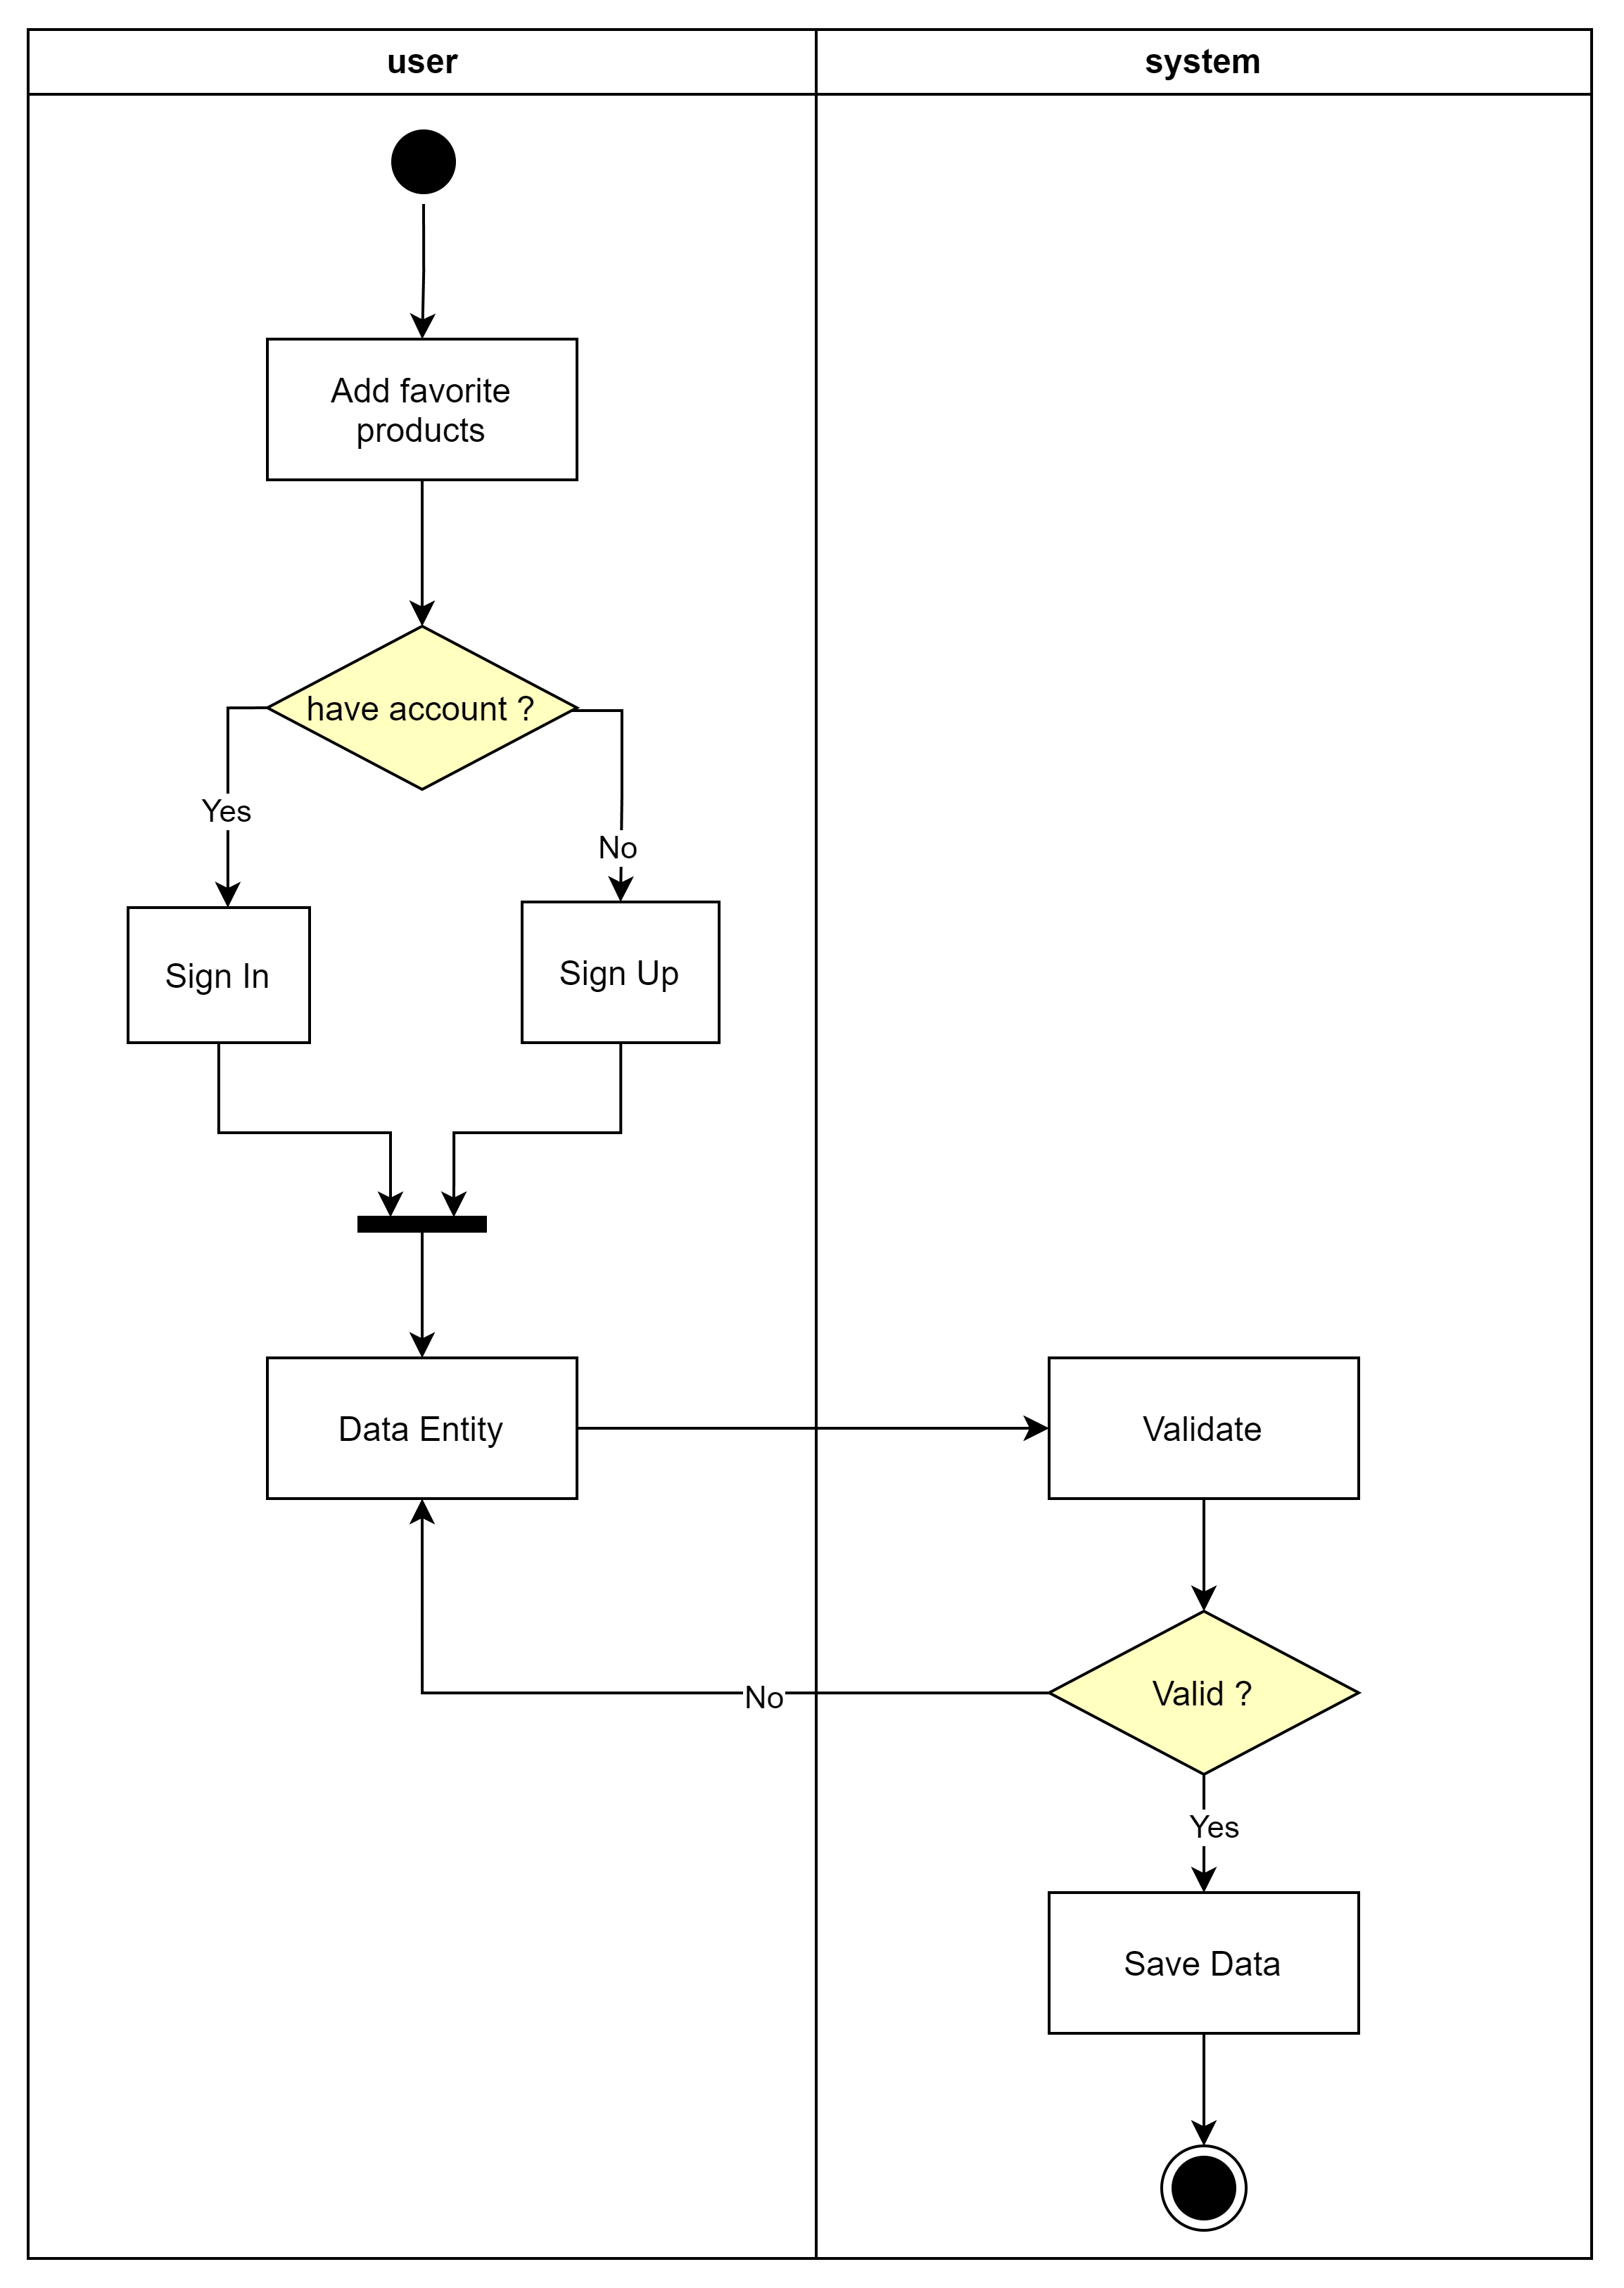
\includegraphics[scale = 0.12]{img/activity/favori.png}
    \vspace{1cm}
    \caption{Activity diagram cho chức năng thêm sản phẩm yêu thích}
    \label{fig:taskAssignment}
\end{figure}

\newpage
\begin{figure}[h]
    \centering
    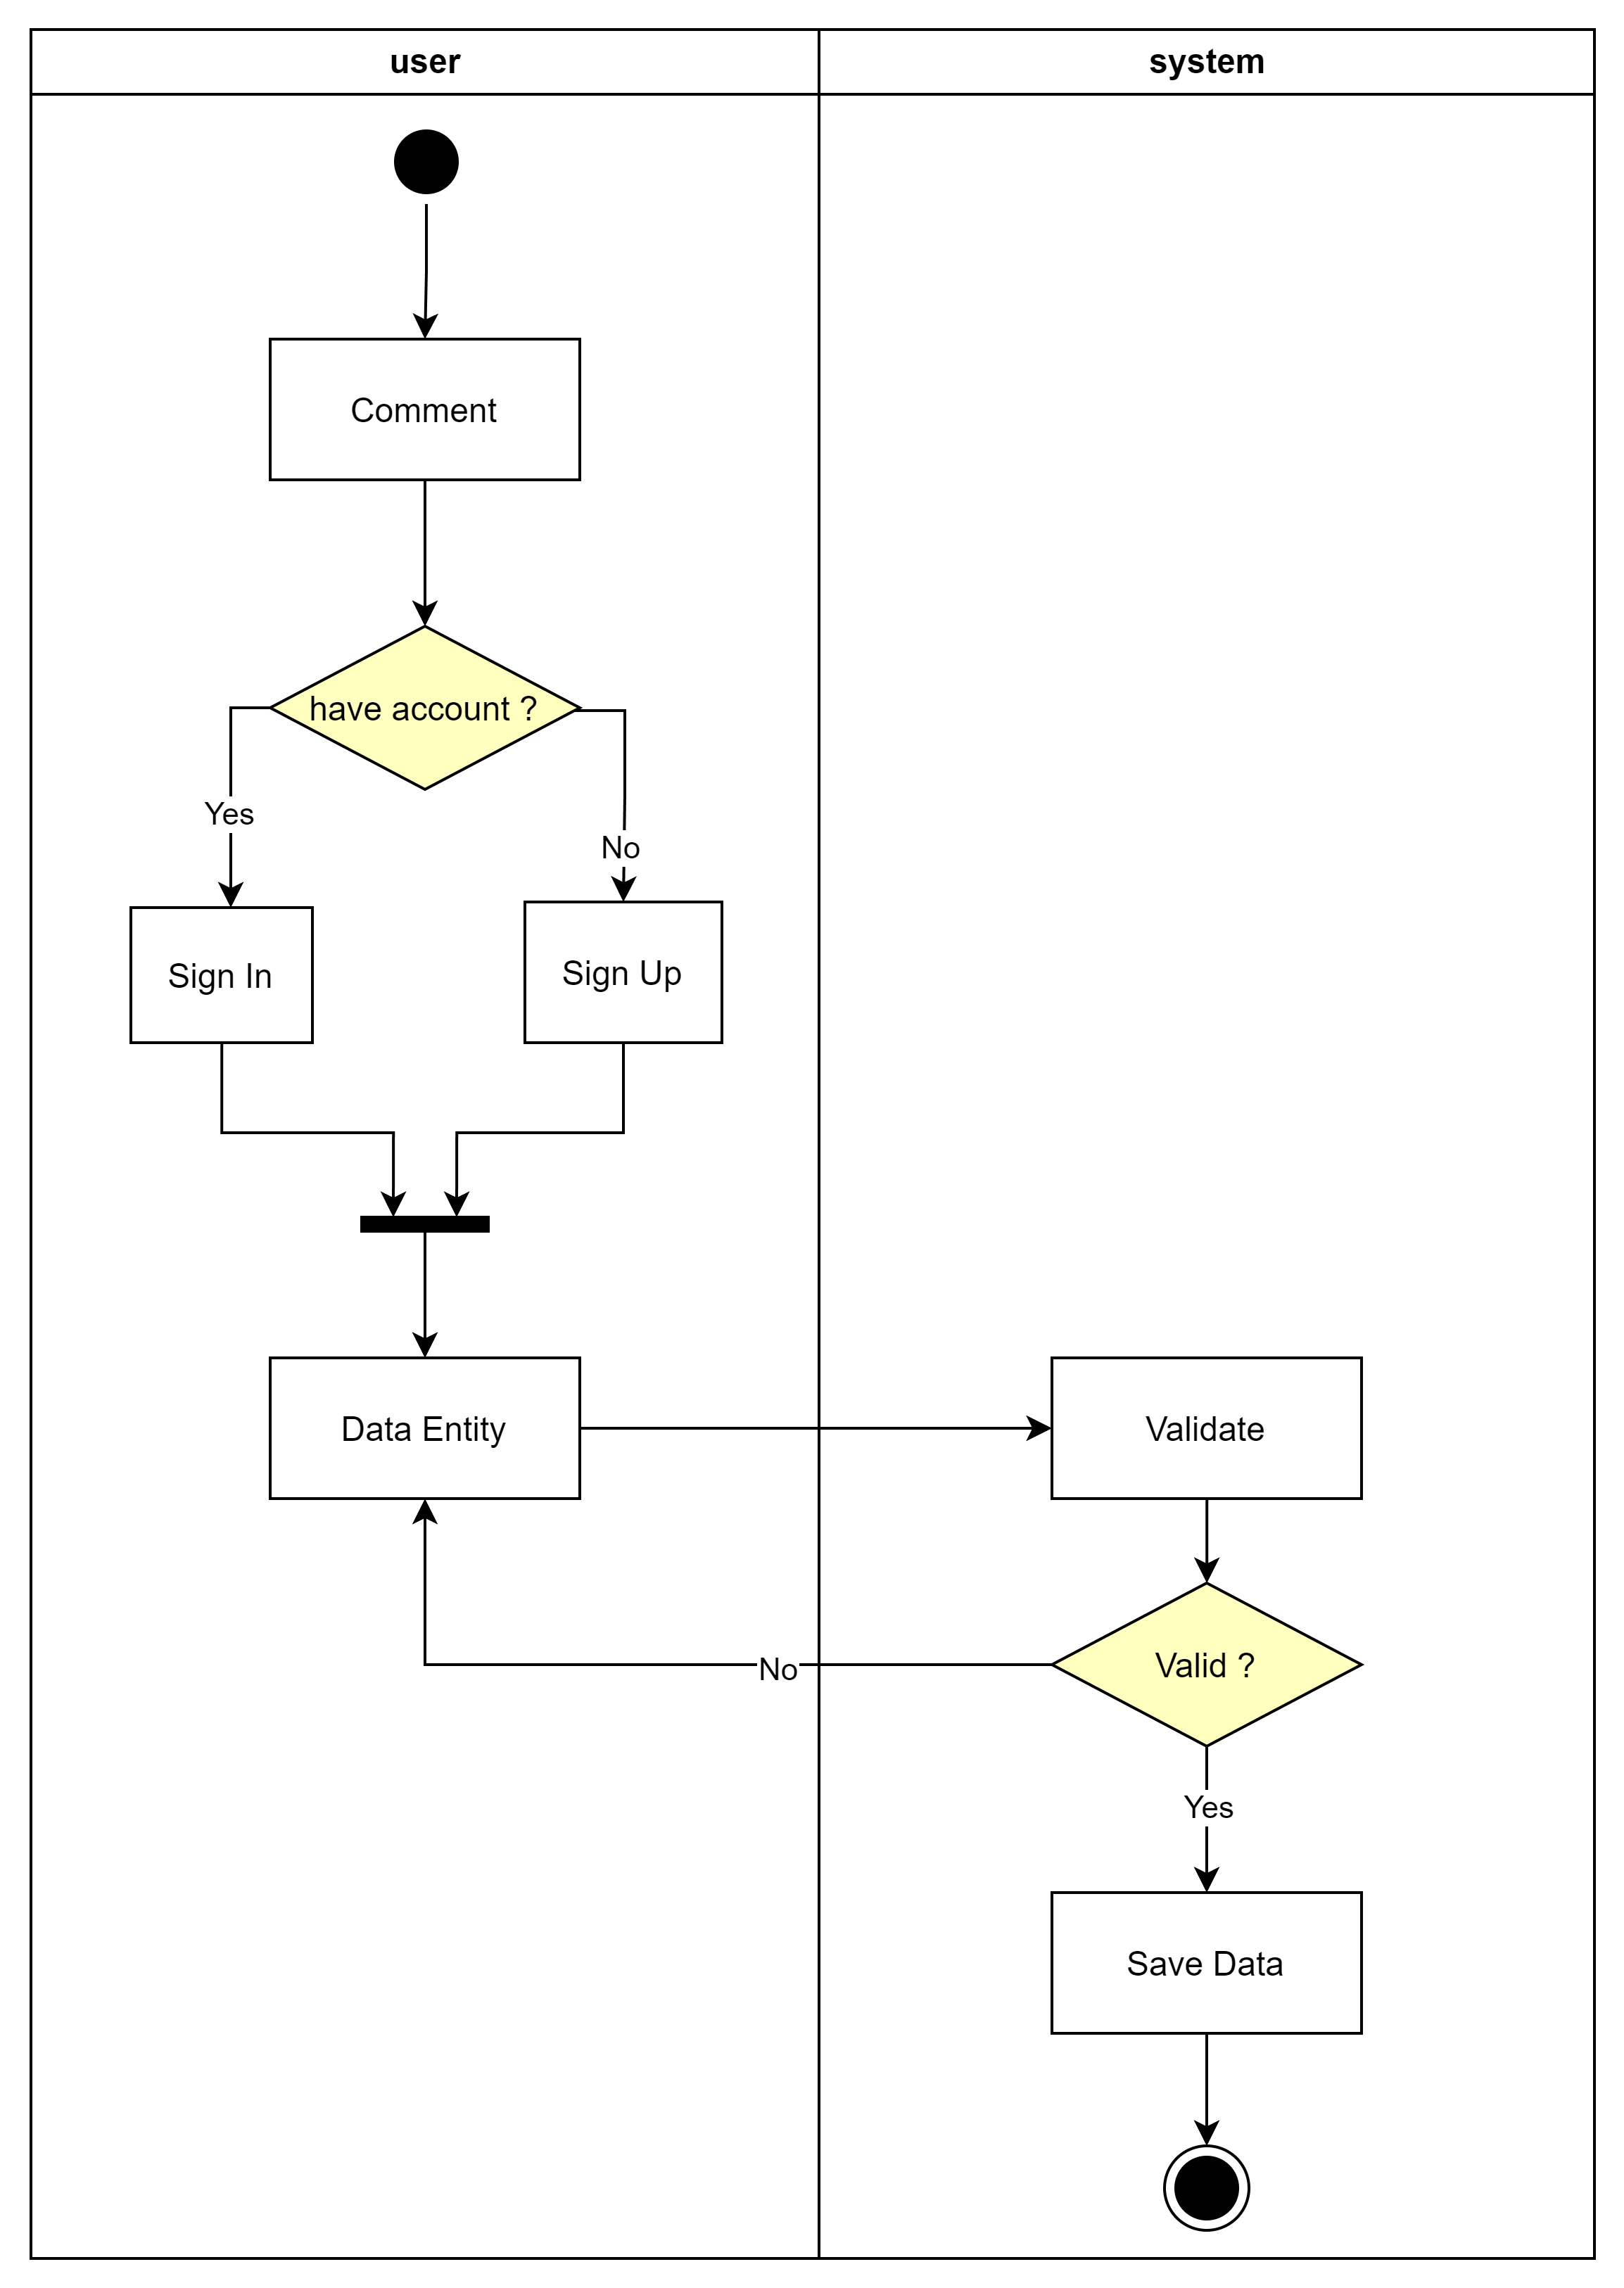
\includegraphics[scale = 0.12]{img/activity/comment.png}
    \vspace{1cm}
    \caption{Activity diagram cho chức năng bình luận}
    \label{fig:taskAssignment}
\end{figure}